\chapter {Element Attributes}
\label{c:attrib}
\index{element attribute}

For a listing of element attributes for each type of element, see Chapter~\sref{c:attrib.list}.

%-----------------------------------------------------------------
\section{Dependent and Independent Attributes} 
\label{s:depend} 
\index{element attribute!dependent and independent}

\index{parameter statement}
\index{dependent attribute}
For convenience, \bmad computes the values of some attributes based upon the values of
other attributes. Some of these dependent variables are listed in
Table~\ref{t:dependent}. Also shown in Table~\ref{t:dependent} are the independent
variables they are calculated from.  In the table \vn{n_part} and \vn{l_lattice} (lattice
length) are lattice attributes, not element attributes. The first two are set by the
\vn{parameter} statement (See \sref{s:param}). \vn{l_lattice} is calculated when the
lattice is read in.

\index{bbi_constant}\index{charge}\index{sig_x}\index{sig_y}
\index{e_tot}\index{n_part}\index{e_field}\index{voltage}
\index{hkick}\index{vkick}\index{gap}\index{l}
\index{e_tot}\index{e_loss}\index{delta_e}\index{gradient}
\index{l}\index{rho}\index{angle}\index{l_chord}
\index{g}\index{l}\index{k1}\index{rho}\index{num_steps}\index{ds_step}
\index{b_max}\index{e_tot}\index{beambeam}\index{elseparator}
\index{lcavity}\index{rbend}\index{sbend}\index{wiggler}
\begin{table}[ht]
\centering {
\begin{tabular}{lll} \toprule
 {\em Element}                & {\em Independent Variables}    & {\em Dependent Variables}          \\ \midrule
 All elements                 & \vn{ds_step}                   & \vn{num_steps}                     \\
 \vn{BeamBeam}                & \vn{charge}, \vn{sig_x}, \vn{sig_y}, \vn{e_tot}, \vn{n_part}
                                                               & \vn{bbi_constant}                  \\
 \vn{Elseparator}             & \vn{hkick}, \vn{vkick}, \vn{gap}, \vn{l}, \vn{e_tot}      
                                                               & \vn{e_field}, \vn{voltage}         \\
 \vn{Lcavity}                 & \vn{gradient}, \vn{l}          & \vn{e_loss}, \vn{voltage}          \\
 \vn{Rbend}, \vn{Sbend}       & \vn{g}, \vn{l}                     
                                                               & \vn{rho}, \vn{angle}, \vn{l_chord} \\

 \vn{Wiggler} (map type)      & \vn{term(i)}                   & \vn{b_max}, \vn{k1}, \vn{rho}      \\
 \vn{Wiggler} (periodic type) & \vn{b_max}, \vn{e_tot}         & \vn{k1}, \vn{rho}                  \\ \bottomrule
\end{tabular}
}
\caption[Table of dependent variables.]{Partial listing of dependent variables and 
  the independent variables they are calculated from.}
\label{t:dependent}
\end{table}

For electric and magnetic field strength parameters, the \vn{field_master} parameter
(\sref{s:field.master}) can be used to determine if the be normalized or unnormalized,
values are dependent or independent.

\index{lattice!expansion}\index{harmon}\index{delta_e}\index{gradient}
\index{rho}\index{g}\index{angle}\index{rf_frequency}
No attempt should be made to set or vary within a program dependent attributes. It should
be remarked that this is not an iron clad rule.  If a program properly bypasses \bmad's
attribute bookkeeping routine then anything is possible. In a lattice file, before lattice
expansion (\sref{s:expand}), \bmad allows the setting of a select group of dependent
attributes if the appropriate independent attributes are not set. The list of settable
dependent variables is given in Table~\ref{t:dep.except}.  After reading in the lattice
\bmad will set the appropriate independent variable based upon the value of the dependent
variable. \vn{harmon} is the exception in that it will never be set by the bookkeeping
routine.
\index{lcavity}\index{rbend}
\index{sbend}\index{rfcavity}
\begin{table}[ht]
\centering {
\begin{tabular}{lll} \toprule
{\em Element}                  & {\em Dependent Variable Set}  &  {\em Independent Variables Not Set} \\ \midrule
  \vn{Lcavity}                 & \vn{voltage}       & \vn{gradient}      \\
  \vn{Rbend}, \vn{Sbend}       & \vn{rho}           & \vn{g}             \\
  \vn{Rbend}, \vn{Sbend}       & \vn{angle}         & \vn{g}, or \vn{l}  \\
  \vn{RFcavity}                & \vn{rf_frequency}  & \vn{harmon}        \\
  \vn{Wiggler} (periodic type) & \vn{n_pole}        & \vn{l_pole}        \\ \bottomrule
\end{tabular}
}
\caption {Dependent variables that can be set in a primary lattice file.}
\label{t:dep.except}
\end{table}

%-----------------------------------------------------------------
\section{Field_Master}
\label{s:field.master}
\index{field_master}

The \vn{field_master} attribute of an element sets whether the element's normalized
(normalized by the reference energy) field strengths or the unnormalized strengths are the
independent variables (\sref{s:depend}).  The setting of \vn{field_master} also sets
whether an element's magnetic multipoles (\sref{s:multip}) are interpreted as normalized or
unnormalized (electric multipoles are always treated as unnormalized).

Table~\ref{t:dep.field} shows some normalized and unnormalized field strength attributes.
The default value of \vn{field_master} for an element is False if there are no field
values set in the lattice file for that element. If normalized field values are present
then the default is also False and if there are unnormalized field values present then
the default is True.

For example:
\begin{example}
  Q1: quadrupole, b1_gradient = 0   ! Field strengths are the independent variables
  Q1: quadrupole, field_master = T  ! Same as above
  Q2: quadrupole        ! Define Q2.
  Q2[b1_gradient] = 0   ! Field strengths now the independent variables.
  Q2[field_master] = T  ! Same as above.
\end{example}

Specifying both normalized and unnormalized strengths for a given element is not
permitted. For example:
\begin{example}
  Q3: quadrupole, k1 = 0.6, bl_hkick = 37.5  ! NO. Not VALID.
\end{example}

\index{g}\index{g_err}\index{b_field}\index{bs_field}\index{b_field_err}
\index{b1_gradient}\index{b2_gradient}\index{b3_gradient}\index{ks}
\index{k1}\index{k2}\index{k3}
\index{bl_kick}\index{bl_hkick}\index{bl_vkick}
\index{kick}\index{hkick}\index{vkick}
\index{sbend}\index{rbend}\index{solenoid}\index{quadrupole}
\index{sol_quad}\index{sextupole}\index{octupole}
\begin{table}[ht]
\centering {
\begin{tabular}{lll} \toprule
  {\em Element}              & {\em Normalized} & {\em Unnormalized}   \\ \midrule
  \vn{Sbend}, \vn{Rbend}     & \vn{g}           &  \vn{b_field}        \\
  \vn{Sbend}, \vn{Rbend}     & \vn{g_err}       &  \vn{b_field_err}    \\
  \vn{Solenoid, Sol_quad}    & \vn{ks}          &  \vn{bs_field}       \\
  \vn{Quadrupole, Sol_quad, Sbend, Rbend}            
                             & \vn{k1}          &  \vn{b1_gradient}    \\
  \vn{Sextupole, Sbend, Rbend}             
                             & \vn{k2}          &  \vn{b2_gradient}    \\
  \vn{Octupole}              & \vn{k3}          &  \vn{b3_gradient}    \\
  \vn{HKicker}, \vn{VKicker} & \vn{kick}        &  \vn{bl_kick}        \\
  Most                       & \vn{hkick}       &  \vn{bl_hkick}       \\
  Most                       & \vn{vkick}       &  \vn{bl_vkick}       \\ \bottomrule
\end{tabular}
}
\caption {Example normalized and unnormalized field strength attributes.}
\label{t:dep.field}
\end{table}

%-----------------------------------------------------------------
\section{Type, Alias and Descrip Attributes}
\label{s:alias}
\index{type|hyperbf}
\index{alias|hyperbf}
\index{descrip|hyperbf}

There are three string labels associated with any element:
\begin{example}
  type    = <String>
  alias   = <String>
  descrip = <String>
\end{example}
\bmad routines do not use these labels except when printing element
information. \vn{type} and \vn{alias} can be up to 40 characters in
length and \vn{descrip} can be up to 200 characters. The attribute
strings can be enclosed in double quotation marks ("). The attribute
strings may contain blanks. If the attribute string does not contain a
blank then the quotation marks may be omitted. In this case the first
comma (,) or the end of the line marks the end of the string. Example:
\begin{example}
  Q00W: Quad, type = "My Type", alias = Who_knows, &
                                  descrip = "Only the shadow knows"
\end{example}

%-----------------------------------------------------------------
\section{Syntax for Group and Overlay Elements}
\label{s:go.syntax}
\index{group!syntax}\index{overlay!syntax}
\index{gang|hyperbf}

The syntax for specifying \vn{group} (\sref{s:group}) and \vn{overlay} (\sref{s:overlay}) elements
are virtually identical and is discussed below. The name ``\vn{controller}'' will be used to denote
either a \vn{group} or \vn{overlay} element.

Controller elements have a set of one or more ``\vn{variables}'' that are used to control the values
of attributes of other elements (called ``\vn{slave}'' attributes).

There are two types of controllers. \vn{Expression} based controllers and \vn{Spline} based
controllers. \vn{Expression} based controllers use mathematical expressions to define how slave
attribute values are calculated based upon the values of the controller variables. \vn{Spline} based
controllers use a spline fit (in particular, the cubic non-smoothing Akima
spline\cite{b:akima}) to a function defined by a set of points (called ``\vn{knots}'') to
determine the relationship between variables and slave attributes. With a spline based controller,
the number of variables is restricted to be one. 

The general syntax for an expression based \vn{group} element is
\begin{example}
  name: GROUP = \{ele1[attrib1]:exp1, ele2[attrib2]:exp2, ...\}, 
          VAR = \{var1, var2, ...\}, var1 = init_val1, 
          old_var1 = old_init_val1, GANG = logical, ...
\end{example}
For an  expression based \vn{overlay} element the syntax is identical except OVERLAY is
substituted for GROUP and there are no old values to set:
\begin{example}
  name: OVERLAY = \{ele1[attrib1]:exp1, ele2[attrib2]:exp2, ...\}, 
          VAR = \{var1, var2, ...\}, var1 = init_val1, GANG = logical, ...
\end{example}
\vn{Name} is the name of the controller element, \vn{ele1}, \vn{ele2},
... are the elements whose attributes are to be controlled,
\vn{attrib1}, \vn{attrib2}, etc. are the controlled attributes (called
``slave'' attributes), \vn{var1}, \vn{var2}, etc. are the control
variables, and \vn{exp1}, \vn{exp2}, etc. are the arithmetical
expressions that define the relationship between the variables and the
slave attributes. Example:
\begin{example}
  gr1: group = \{q1[k1]:-tan(a)*b, q2[tilt]:b^2\}, var = \{a, b\}
\end{example}

To define an expression based \vn{controller} element, two lists are needed: One list
defines the slave attributes along with the arithmetic expressions
used for computing the value of the slave attributes. The other list
defines the variables within the \vn{controller} element that can be
varied. In the above example, the variables are \vn{a} and \vn{b}, and
the slave attributes are the \vn{k1} attribute of element \vn{q1} and
the \vn{tilt} attribute of element \vn{q2}. The arithmetic expressions
used for the control are \vn{-tan(a)*b} and \vn{b\^{}2}.

The general syntax for For a \vn{spline} based \vn{group} element is
\begin{example}
  name: GROUP = \{ele1[attrib1]:\{y_knot_points1\}, ele2[attrib2]:\{y_knot_points2\}, ...\}, 
              VAR = \{var1\}, X_KNOT = \{x_knot_points\},
              var1 = init_val1, old_var1 = init_val_old1, ...
\end{example}
and the general syntax for a \vn{spline} based  \vn{overlay} element is
\begin{example}
  name: OVERLAY = \{ele1[attrib1]:\{y_knot_points1\}, ele2[attrib2]:\{y_knot_points2\}, ...\}, 
              VAR = \{var1\}, X_KNOT = \{x_knot_points\}, var1 = init_val1, ...
\end{example}
Example:
\begin{example}
  ov: overlay = \{q1[k1]:\{0.234, 0.534\}, q2[k1], q3[k1], q4[k1]:\{0.375, 0.923\}\}, 
        var = {time}, x_knot = \{0.0, 1.0\}
\end{example}
The array sizes of all knot arrays must be the same. If a \vn{y_knot_points} array is not present
for a particular slave attribute, the knot array of the previous slave attribute is used. Thus, in
the above example, the y_knot array used for \vn{q2[k1]} and \vn{q3[k1]} are the same as the y_knot
array for \vn{q1[k1]}.

If the \vn{gang} attribute is \vn{True} (which is the default) a \vn{controller} will
control all elements of a given name. Thus, in the above example, if there are multiple
elements named \vn{q1} then \vn{gr1} will control the \vn{k1} attribute of all of them.
If \vn{gang} is set to \vn{False}, then a separate controller is created for each element
in the lattice of a given name. For example:
\begin{example}
  gr1: group = \{q1[k1]:-tan(a)*b, q2[tilt]:b^2\}, var = \{a, b\}, gang = False
\end{example}
In this example, suppose there are five \vn{q1} and five \vn{q2} elements in the lattice.
In this case, there will be five \vn{gr1} group elements created. The first \vn{gr1} will
control the first \vn{q1} and \vn{q2} to appear in the lattice, etc. With \vn{gang} set to
\vn{False}, it is an error if the number of instances in the lattice for a given slave
name is different from any other slave name. In this example, it would be an error if the
number of \vn{q1} elements in the lattice is different from the number of \vn{q2} elements
in the lattice.

The syntax for specifying an attribute \vn{attrib} of element \vn{ele}
to be controlled is \vn{ele[attrib]}. The attribute part \vn{[attrib]}
may be omitted and in this case the name of the attribute will be
taken to be the name of the first variable. Example:
\begin{example}
  ov1: overlay = \{sex1:-tan(k2)^b\}, var = \{k2, b\}
\end{example}
In this example, the controlled attribute of element \vn{sex1} is
\vn{k2}.  Except in cases where this default attribute syntax is used,
the names of the variables are arbitrary and do not have to correspond
to the name of any actual attribute.

The arithmetic expressions used to evaluate controlled attribute value
changes may be a constant. In this case, the actual expression used is
this constant times the first variable. If the expression is omitted
entirely, along with the separating ``:'', the constant will be taken
to be unity. Example:
\begin{example}
  gr1: group = \{b1, b3:-pi\}, var = \{angle\}
\end{example}
This is equivalent to
\begin{example}
  gr1: group = \{b1[angle]:angle, b3[angle]:-pi*angle\}, var = \{angle\}
\end{example}

Arithmetic expressions may themselves contain element attributes.
Example:
\begin{example}
  sk_q20W: overlay = \{sex_20W[a1]:-sex_20W[L]\}, k1
\end{example}
Here the \vn{sk_q20w} overlay controls the \vn{a1} multipole attribute of element
\vn{sex_20w} and the length of \vn{sex_20w} is used as a scale factor between the
overlay's variable \vn{k1} and the controlled attribute \vn{a1}. The potential problem
here is that, to keep the internal bookkeeping simple, the value of \vn{sex_20w[L]} is
evaluated once during parsing of the lattice file and never reevaluated (\sref{s:arith}).
If it is desired to use a variable element attribute in an expression, this may be
effectively done by defining a control variable to take its place. Thus the above overlay
may be recast as:
\begin{example}
  sk_q20W: overlay = \{sex_20W[L]:ll, sex_20W[a1]:ll*k1\}, var = \{k1, ll\}
\end{example}

Initial values can be assigned to the variables from within the
definition of the controller element. Example:
\begin{example}
  ov1: overlay = \{...\}, var = \{a, b\}, a = 7, b = 2
\end{example}
Here the initial values 7 and 2 are assigned to \vn{a} and \vn{b} respectively.
Alternatively, variables can be set after a controller element has been defined. 
Example:
\begin{example}
  ov1: overlay = \{...\}, var = \{a, b\}
  ov1[a] = 7
  gr1[b] = 2
\end{example}

There is an old deprecated syntax. For \vn{group} elements the syntax was:
\begin{example}
  name: GROUP = \{ele1[attrib1]:coef1, ele2[attrib2]:coef2, ...\}, 
                       attrib = init_value  ! DO NOT USE THIS SYNTAX!
\end{example}
and for \vn{overlay} elements the old syntax was identical except
that \vn{GROUP} was replaced by \vn{OVERLAY}:
\begin{example}
  name: OVERLAY = \{ele1[attrib1]:coef1, ele2[attrib2]:coef2, ...\}, 
                       attrib = init_value  ! DO NOT USE THIS SYNTAX!
\end{example}

With this old syntax, there is only one variable. Additionally, there
are no arithmetic expressions. Rather, attribute changes are linear in
the \vn{command} variable with the constant of proportionality given
by a specified coefficient. For example with the old syntax
\begin{example}
  ov1: overlay = \{sq1:3.7, sq2[tilt]\}, k0 = 2  ! DO NOT USE THIS SYNTAX!
\end{example}
is equivalent, in the present syntax, to:
\begin{example}
  ov1: overlay = \{sq[k0]:3.7, sq2[tilt]\}, var = \{k0\}, k0 = 2  
\end{example}
Note: In this old syntax the colon ``:'' separating the controlled
attribute from the linear coefficient may be replaced by a slash
``/''.  For \vn{group} elements, there was an added wrinkle that, with
the old syntax, the variable's name is fixed to be \vn{command}. For
example, with the old syntax
\begin{example}
  gr1: group = \{sq1:3.7, sq2[tilt]\}, k0 = 2  ! DO NOT USE THIS SYNTAX!
\end{example}
is equivalent, in the present syntax, to:
\begin{example}
  gr1: group = \{sq[k0]:3.7, sq2[tilt]\}, var = \{command\}, command = 2  
\end{example}

%-----------------------------------------------------------------
\section[Energy and Wavelength Attributes]{Energy and Wavelength Attributes: E_tot, P0C, and \\ Ref_Wavelength}
\label{s:energy}
\index{parameter statement}\index{e_tot}
\index{e_tot_start}\index{p0c_start}
\index{patch}\index{lcavity}\index{p0c}\index{e_gun}
\index{n_ref_pass}\index{ref_wave_length}
The attributes that define the reference energy and momentum at an element are:
\begin{example}
  e_tot  = <Real>  ! Total energy in eV.
  p0c    = <Real>  ! Momentum in eV.
\end{example}
The energy and momentum are defined at the exit end of the element.
For ultra--relativistic particles, and for photons, these two values
are the same (\sref{s:phase.space}). Except for multipass elements
(\sref{s:multipass}), \vn{e_tot} and \vn{p0c} are dependent attributes
and, except for multipass elements, any setting of \vn{e_tot} and
\vn{p0c} in the lattice input file is an error. The value of
\vn{e_tot} and \vn{p0c} for an element is calculated by \bmad to be
the same as the previous element except for \vn{e_gun}, \vn{lcavity} and
\vn{patch} elements. To set the \vn{e_tot} or \vn{p0c} at the start of
the lattice use the \vn{beginning} or \vn{parameter} statements.
See~\sref{s:param}. Since the energy changes from the start to the end
of an \vn{lcavity} or. \vn{em_field}, an \vn{lcavity} or \vn{em_field} has
the dependent attributes
\index{em_field}\index{lcavity}
\begin{example}
  e_tot_start   and
  p0c_start
\end{example}
which are just the reference energy and momentum at the start of the element.

\index{beginning_ele}
The \vn{beginning_ele} element (\sref{s:begin.ele}) also has associated
\vn{e_tot_start} and \vn{p0c_start} attributes as well as \vn{e_tot}
and \vn{p0c}. Generally, for an \vn{beginning_ele}, \vn{p0c_start} and
\vn{p0c} are the same and \vn{e_tot_start} and \vn{e_tot} are the same
and the values for these attributes are set in the lattice file with
the appropriate \vn{parameter} (\sref{s:param}) or \vn{beginning}
(\sref{s:beginning}) statement. The exception occurs when there is an
\vn{e_gun} element in the lattice (\sref{s:e.gun}). In this case, the
\vn{p0c_start} and \vn{e_tot_start} attributes of the \vn{beginning_ele}
are set to the values as set in the lattice file and \vn{e_tot} is set
to
\begin{example}
  e_tot = e_tot_start + voltage
\end{example}
and \vn{p0c} is calculated from \vn{e_tot} and the mass of the
particle being tracked. For example, if the lattice file contained:
\begin{example}
  beginning[p0c] = 0
  gun: e_gun, voltage = 0.5e6
  injector: line = (gun, ...)
\end{example}
Then the following energy values will be set for the beginning \vn{beginning_ele} element:
\begin{example}
  p0c_start   = 0
  e_tot_start = mc2
  e_tot       = mc2 + 0.5e6
  p0c         = Sqrt(e_tot - mc2^2)
\end{example}
where \vn{mc2} is the particle rest mass.  The reason for using this
convoluted convention is to allow the setting, in the lattice file, of
a zero reference momentum at the start of the lattice, while
avoiding the calculational problems that would occur if the \vn{e_gun}
element truly had a starting reference momentum of zero.
Specifically, the problem with zero reference momentum is that the
phase space momentum would be infinity as can be seen from \Eqs{ppp}.

For \vn{multipass} elements, the reference energy is set by specifying
one of \vn{e_tot}, \vn{p0c}, or \vn{n_ref_pass} as described in
\sref{s:multipass}.

For photons, the reference wavelength, \vn{ref_wavelength} is also a
dependent attribute calculated from the reference energy.

\vfill

%-----------------------------------------------------------------
\section{Orientation: Offset, Pitch, Tilt, and Roll Attributes}
\label{s:offset}
\index{x_offset|hyperbf}
\index{y_offset|hyperbf}\index{z_offset|hyperbf}
\index{x_pitch|hyperbf}\index{y_pitch|hyperbf}
\index{roll|hyperbf}\index{tilt|hyperbf}

By default, an element, like a quadrupole, is aligned in space
coincident with the reference orbit running through it
(\sref{s:ref.construct}). A quadrupole can be displaced in space using
the quadrupole's ``\vn{orientational}'' attributes. For a quadrupole,
the orientational attributes only affect the physical element and not
the reference orbit. However, the orientational attributes of some
other elements, like the \vn{fiducial} element, do affect the
reference orbit. To sort all this out, lattice elements can be divided
into seven classes:
  \begin{enumerate}
  \item\vn{Straight line elements} (\sref{s:straight.orient}) \Newline
Straight line elements are elements where the reference orbit is a
straight line. Examples include \vn{quadrupoles}, and \vn{sextupoles}
as well as zero length elements like \vn{markers}.
  \item\vn{Dipole bends} (\sref{s:bend.orient}) \Newline
Dipole bends are:
\begin{example}
  sbend \& rbend
\end{example}
  \item\vn{Photon reflecting elements} (\sref{s:photon.orient}) \Newline
The reflecting elements are
\begin{example}
  crystal
  mirror
  multilayer_mirror
\end{example}
These elements have a kink in the reference orbit at the nominal
element surface.
  \item\vn{Reference orbit manipulator elements} (\sref{s:manip.orient}) \Newline
Elements that are used to manipulate the reference orbit are
\begin{example}
  fork \& photon_fork
  floor_shift
  patch
\end{example}
  \item\vn{Fiducial Element} (\sref{s:fiducial.orient}) \Newline
  \item\vn{Girder Elements} (\sref{s:girder.orient}) \Newline
  \item\vn{Control Elements} \Newline
Control elements are elements that control attributes of other
elements. The control elements are:
\begin{example}
  group
  overlay
\end{example}
These elements do not have orientational attributes.
  \end{enumerate}

%-----------------------------------------------------------------
\subsection{Straight Line Element Orientation}
\label{s:straight.orient}

The straight line elements have the following orientational attributes:
\begin{example}
  x_offset = <Real>
  y_offset = <Real>
  z_offset = <Real>
  x_pitch  = <Real>
  y_pitch  = <Real>
  tilt     = <Real>    
\end{example}
For straight line elements the orientational attributes only shift the
physical element and do not affect the reference orbit.

\begin{figure}[tb]
  \centering
  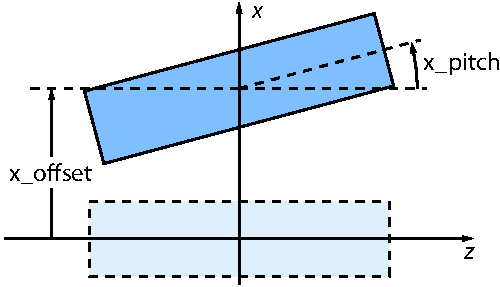
\includegraphics{pitch.pdf}
  \caption{Geometry of Pitch and Offset attributes}
  \label{f:pitch}
\end{figure}

\vn{x_offset} translates an element in the local $x$--direction
as shown in \fig{f:pitch}. Similarly, \vn{y_offset} and 
\vn{z_offset} translate an element along the local $y$ and 
$z$--directions respectively.

The \vn{x_pitch} attribute rotates an element about the element's center such that with a positive
\vn{x_pitch} the exit face of the element is displaced in the $+x$--direction as shown in
figure~\ref{f:pitch}. [One way to visualize the effect of an \vn{x_pitch} is to think of the element
as an airplane pointing in the $+z$ direction. A positive \vn{x_pitch} would then move the front of
the plane in the $+x$--direction.] An\vn{x_pitch} represents a rotation around the positive
$y$-axis.

Similarly, the \vn{y_pitch} attribute rotates an element about the element's center using the
negative $x$--axis as the rotation axis so that, with a positive \vn{y_pitch} the exit face of the
element is displaced in the $+y$--direction.

Note: the \vn{x_pitch} and \vn{y_pitch} rotations are about the center of the element which is in contrast
to the \vn{dtheta} and \vn{dphi} misalignments of \mad which rotate around the entrance point. The
sense of the rotation between \bmad and MAD is:
\index{MAD!element rotation origin}
\begin{example}
  x_pitch (Bmad) =  dtheta (MAD)
  y_pitch (Bmad) = -dphi (MAD)
\end{example}

\begin{figure}[tb]
  \centering
  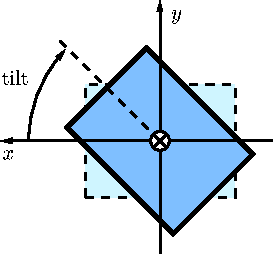
\includegraphics{tilt.pdf}
  \caption{Geometry of a Tilt}
  \label{f:tilt}
\end{figure}

The tilt attribute rotates the element in the $(x, y)$ plane as shown
in figure~\ref{f:tilt}. The rotation axis is the positive
$z$-axis. For example
\begin{example}
  q1: quad, l = 0.6, x_offset = 0.03, y_pitch = 0.001, tilt
\end{example}
\index{sol_quad!tilt default}\index{quadrupole!tilt default}
\index{sextupole!tilt default}\index{octupole!tilt default}
Like MAD, \bmad allows the use of the \vn{tilt} attribute without a
value to designate a skew element. The default tilt is $\pi/(2(n+1))$
where $n$ is the order of the element:
\begin{example}
  sol_quad       n = 1
  quadrupole     n = 1
  sextupole      n = 2
  octupole       n = 3
\end{example}

Note that \vn{hkick} and \vn{vkick} attributes are not affected by
\vn{tilt} except for \vn{kicker} and \vn{elseparator} elements.

%-----------------------------------------------------------------
\subsection{Bend Element Orientation}
\label{s:bend.orient}

\begin{figure}[ht]
  \centering
  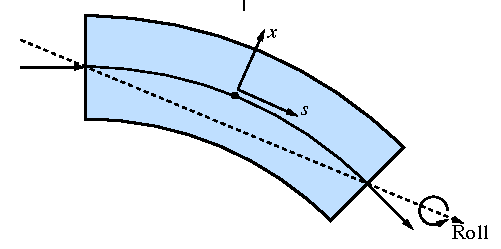
\includegraphics{roll.pdf}
  \caption[Geometry of a Bend]{
Geometry of a Bend. Like straight line elements, offsets and pitches
are calculated with respect to the coordinates at the center of the
bend. The exception is the \vn{roll} attribute which is a rotation
around the axis passing through the entrance and exit points.  Shown
here is the geometry for a bend with \vn{ref_tilt} = 0. That is, the bend
is in the $x-z$ plane.}
  \label{f:roll}
\end{figure}

The orientation attributes for \vn{sbend} and \vn{rbend} elements is
\begin{example}
  x_offset = <Real>
  y_offset = <Real>
  z_offset = <Real>
  x_pitch  = <Real>
  y_pitch  = <Real>
  ref_tilt = <Real>    ! Shifts and reference orbit rotation axis.
  roll     = <Real>    
\end{example}
The geometry for orienting a bend is shown in \fig{f:roll}. Like
straight line elements, the offset and pitch attributes are evaluated
with respect to the center of the element. 

Unlike the straight line elements, bends do not have a \vn{tilt}
attribute. Rather they have a \vn{ref_tilt} and a \vn{roll} attribute.
The \vn{roll} attribute rotates the bend along an axis that runs
through the entrance point and exit point as shown in
figure~\ref{f:roll}. A \vn{roll} attribute, like the offset and pitch
attributes does not affect the reference orbit.
The major effect of a \vn{roll} is to give a vertical
kick to the beam. For a bend with positive bend angle, a positive
\vn{roll} will move the outside portion ($+x$ side) of the bend upward
and the inside portion (-$x$ side) downward. Much like car racetracks
which are typically slanted towards the inside of a turn.

The \vn{ref_tilt} attribute of a bend rotates the bend about the $z$
axis at the upstream end of the bend as shown in \fig{f:roll}. Unlike
\vn{rolls} and \vn{tilts}, \vn{ref_tilt} also shifts the rotation axis
of the reference orbit along with the physical element. A \vn{bend}
with a \vn{ref_tilt} of $\pi/2$ will bend a beam vertically downward
(\sref{s:global}). Note that the \vn{ref_tilt} attribute of \bmad is
the same as the MAD \vn{tilt} attribute.

%-----------------------------------------------------------------
\subsection{Photon Reflecting Element Orientation}
\label{s:photon.orient}

\begin{figure}[ht]
  \centering
  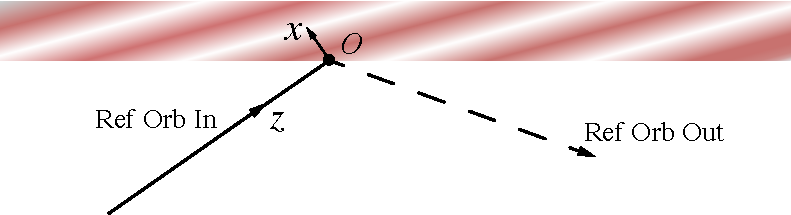
\includegraphics{reflect-orient.pdf}
  \caption[Geometry of a photon reflecting element orientation]{
Geometry of a photon reflecting element orientation.
The reference coordinates used for defining the orientational attribute
is the entrance reference coordinates. 
}
  \label{f:reflect.orient}
\end{figure}

Photon reflecting elements have the following orientational attributes:
\begin{example}
  x_offset = <Real>
  y_offset = <Real>
  z_offset = <Real>
  x_pitch  = <Real>
  y_pitch  = <Real>
  ref_tilt = <Real>    ! Shifts both element and reference orbit.
  tilt     = <Real>    
\end{example}
Roughly, these elements can be viewed as zero length bends except,
since there is no center position, the orientational attributes are
defined with respect to the entrance coordinates as shown in
\fig{f:reflect.orient}. Like bend elements, the \vn{ref_tilt} attribute
rotates both the physical element and the reference coordinates.
The \vn{tilt} attribute rotates just the physical element. Thus
the total rotation of the physical element about the entrance $z$
axis is the sum \vn{tilt} + \vn{ref_tilt}.

Frequently, it is desired to orient reflecting elements with respect
to the element's surface. This can be done using a \vn{girder} element
(\sref{s:girder}) which supports the reflecting element and with the
\vn{girder}'s \vn{origin_ele_ref_pt} attribute set to \vn{center}.

%-----------------------------------------------------------------
\subsection{Reference Orbit Manipulator Element Orientation}
\label{s:manip.orient}

The \vn{fork}, \vn{photon_fork}, \vn{floor_shift}, and \vn{patch} elements
use the following attributes to orient their exit edge with respect to their
entrance edge:
\begin{example}
  x_offset = <Real>
  y_offset = <Real>
  z_offset = <Real>
  x_pitch  = <Real>
  y_pitch  = <Real>
  tilt     = <Real>    
\end{example}
Here "exit" edge for \vn{fork} and \vn{photon_fork} elements is defined
to be the start of the line being branched to. [Within the line containing
the fork, the \vn{fork} element is considered to have zero length so the exit face
in the line containing the fork is coincident with the entrance face.]
The placement of the exit edge for these elements defines the reference orbit.
Thus, unlike the corresponding attributes for other elements, 
the orientational attributes here directly control the reference orbit.

%-----------------------------------------------------------------
\subsection{Fiducial Element Orientation}
\label{s:fiducial.orient}

The \vn{fiducial} element (\sref{s:girder}) uses the 
following attributes to define its position:
\begin{example}
  origin_ele        = <Name>     ! Reference element.
  origin_ele_ref_pt = <location> ! Reference pt on reference ele.
  dx_origin         = <Real>     ! x-position offset
  dy_origin         = <Real>     ! y-position offset
  dz_origin         = <Real>     ! z-position offset
  dtheta_origin     = <Real>     ! orientation angle offset.
  dphi_origin       = <Real>     ! orientation angle offset.
  dpsi_origin       = <Real>     ! orientation angle offset.
\end{example}
See Section~\sref{s:fiducial} for more details.

%-----------------------------------------------------------------
\subsection{Girder Orientation}
\label{s:girder.orient}

A \vn{girder} (\sref{s:girder}) element uses the same attributes as a \vn{fiducial}
element (\sref{s:fiducial}) to orient the reference girder position. In addition,
the following attributes are used to move the girder physically from the reference position: 
\begin{example}
  x_offset = <Real>
  y_offset = <Real>
  z_offset = <Real>
  x_pitch  = <Real>
  y_pitch  = <Real>
  tilt     = <Real>    
\end{example}
Shifting the girder from its reference position shifts all the elements that are
supported by the girder. See Section~\sref{s:girder} for more details.

\index{x_offset_tot|hyperbf}\index{y_offset_tot|hyperbf}\index{z_offset_tot|hyperbf}
\index{x_pitch_tot|hyperbf}\index{y_pitch_tot|hyperbf}
\index{tilt_tot|hyperbf}\index{roll_tot|hyperbf}\index{tilt_err_tot|hyperbf}
If an element is supported by a \vn{girder} element (\sref{s:girder}),
the orientational attributes of the element are with respect to the
orientation of the \vn{girder}. The computed offsets, pitches and tilt with
respect to the local reference coordinates are stored in the dependent attributes
\begin{example}
  x_offset_tot
  y_offset_tot
  z_offset_tot
  x_pitch_tot
  y_pitch_tot
  tilt_tot
  roll_tot
\end{example}
\index{sbend}\index{rbend}
A \vn{*_tot} attribute will only be present if the corresponding non
\vn{*_tot} attribute is present. For example, only \vn{sbend} and
\vn{rbend} elements have a \vn{roll_tot} attribute since only these
elements have a \vn{roll} attribute.

If an element is not supported by a \vn{girder}, the values of the
\vn{*_tot} attributes will be the same value as the values of the
corresponding non \vn{*_tot} attributes.

%-----------------------------------------------------------------
\section{Hkick, Vkick, and Kick Attributes}
\label{s:kick}
\index{hkick|hyperbf}\index{bl_hkick|hyperbf}
\index{vkick|hyperbf}\index{bl_vkick|hyperbf}
\index{kick|hyperbf}\index{bl_kick|hyperbf}


\index{hkicker}
\index{vkicker}
\index{elseparator}
\index{kicker}
The kick attributes that an element may have are:
\begin{example}
  kick,  bl_kick  = <Real>  ! Used only with a Hkicker or Vkicker
  hkick, bl_hkick = <Real>
  vkick, bl_vkick = <Real>
\end{example}
\vn{kick}, \vn{hkick}, and \vn{vkick} attributes are the integrated
kick of an element in radians. \vn{kick} is only used for \vn{hkicker}
and \vn{vkicker} elements. All other elements that can kick use
\vn{hkick} and \vn{vkick}. The \vn{tilt} attribute will only rotate a
kick for \vn{hkicker}, \vn{vkicker}, \vn{elseparator} and \vn{kicker}
elements. This rule was implemented so that, for example, the
\vn{hkick} attribute for a skew quadrupole would represent a
horizontal steering. The \vn{bl_kick}, \vn{bl_hkick}, and
\vn{bl_vkick} attributes are the integrated field kick in
\vn{meters-Tesla}. Normally these are dependent attributes except if
they appear in the lattice file (\sref{s:depend}).

For an \vn{elseparator} element, the \vn{hkick} and \vn{vkick} are
appropriate for a positively charged particle. The kick for a
negatively charged particle is opposite this.

%-----------------------------------------------------------------
\section{Aperture and Limit Attributes}
\label{s:limit}
\index{aperture|hyperbf}
\index{limit|hyperbf}
\index{aperture_at|hyperbf}

\begin{figure}[ht]
  \centering
  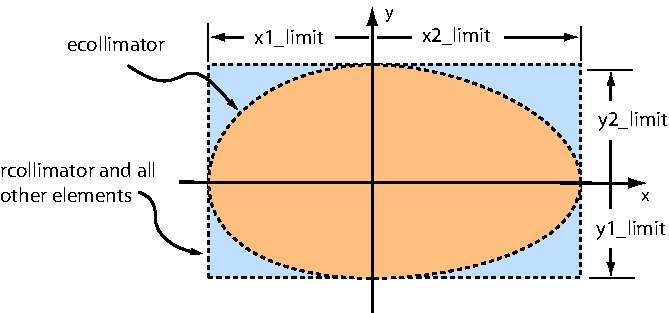
\includegraphics{apertures.pdf}
  \caption[Apertures for ecollimator and rcollimator elements.]
  {Apertures for ecollimator and rcollimator elements. 
  [note: positive $z$ points up, out of the page.] 
  As drawn, all limits \vn{x1_limit}, \vn{x2_limit}, 
  \vn{y1_limit}, \vn{y2_limit} are  positive.}  
  \label{f:limit}
\end{figure}

\index{ecollimator}
\index{rcollimator}
\index{x_limit|hyperbf}
\index{y_limit|hyperbf}
\index{x1_limit|hyperbf}
\index{y1_limit|hyperbf}
\index{x2_limit|hyperbf}
\index{y2_limit|hyperbf}
\index{x_offset|hyperbf}
\index{offset_moves_aperture|hyperbf}
\index{aperture_type}
The aperture attributes are:
\begin{example}
  x1_limit      = <Real>      ! Horizontal, negative side, aperture limit
  x2_limit      = <Real>      ! Horizontal, positive side, aperture limit
  y1_limit      = <Real>      ! Vertical, negative side, aperture limit
  y2_limit      = <Real>      ! Vertical, positive side, aperture limit
  x_limit       = <Real>      ! Alternative to specifying x1_limit and x2_limit
  y_limit       = <Real>      ! Alternative to specifying y1_limit and y2_limit
  aperture      = <Real>      ! Alternative to specifying x_limit and y_limit
  aperture_at   = <Switch>    ! What end aperture is at. (\sref{s:ap.place})
  aperture_type = <Switch>    ! What type of aperture it is
  offset_moves_aperture = <Logical> ! Element offsets affect aperture position (\sref{s:offset.ap})
\end{example}
\vn{x1_limit}, \vn{x2_limit}, \vn{y1_limit}, and \vn{y2_limit} specify
the half--width of the aperture of an element as shown in
figure~\ref{f:limit}. A zero \vn{x1_limit}, \vn{x2_limit},
\vn{y1_limit}, or \vn{y2_limit} is interpreted as no aperture in the
appropriate plane.

For convenience, \vn{x_limit} can be used to set \vn{x1_limit} and
\vn{x2_limit} to a common value. Example:
\begin{example}
  s: sextupole, x1_limit = 0.09, x2_limit = 0.09
  s: sextupole, x_limit = 0.09   ! Same as above
\end{example}
Similarly, \vn{y_limit} can be used
to set \vn{y1_limit} and \vn{y2_limit}.  The \vn{aperture} attribute
can be use to set all four \vn{x1_limit}, \vn{x2_limit}, \vn{y1_limit}
and \vn{y2_limit} to a common value. Internally, the \bmad code does {\em not}
store \vn{x_limit}, \vn{y_limit}, or \vn{aperture}. This means that
using \vn{x_limit}, \vn{y_limit} or aperture in arithmetic expressions is
an error:
\begin{example}
  q1: quad, aperture = 0.09         
  q2: quad, aperture = q1[aperture]   ! THIS IS AN ERROR!
  q2: quad, aperture = q1[x1_limit]   ! Correct
\end{example}

By default, apertures are assumed to be rectangular except that an
\vn{ecollimator} has a elliptical aperture. This can be changed by
setting the \vn{aperture_type} attribute. The possible values of this
attribute are:
\begin{example}
  auto         ! Default for detector, mask and diffraction_plate elements
  custom
  elliptical   ! Default for \vn{ecollimator} elements.
  rectangular  ! Default for most elements.
  wall3d       ! Vacuum chamber wall (\sref{s:wall}).
\end{example}
The \vn{custom} setting is used in the case where programs have been
compiled with custom, non-Bmad, code to handle the aperture
calculation.  The \vn{auto} setting is used for automatic calculation
of a rectangular aperture. For \vn{diffraction_plate} and \vn{mask}
elements, the \vn{auto} setting causes the four aperture limits to be
set to just cover the clear area of element
(\sref{s:masking.wall}). For all other elements, the \vn{auto}
setting is only to be used when there is an associated surface grid
(\sref{s:surf.grid}) for the element and, in this case, \bmad to set
the four limits to just cover the surface grid.

The \vn{wall3d} setting uses the vacuum chamber wall as specified by a \vn{wall} attribute
(\sref{s:wall}). Using the \vn{wall} construct allows for complex apertures to be
constructed. Note that The wall thickness and material type are not used when calculating
if a particle has hit the wall. That is, the wall is considered to be infinitely thin.
Also note that a wall must cover the entire length of the element longitudinally. This is done
in order to be able to spot errors in specifying the wall geometry.

For rectangular apertures, the limits \vn{x1_limit}, \vn{x2_limit},
\vn{y1_limit}, or \vn{y2_limit} may be negative. For example:
\begin{example}
  s: sextupole, x1_limit = -0.02, x2_limit = 0.09
\end{example}
In this case, particles will hit the aperture if their $x$-coordinate
is outside the interval [0.02, 0.09]. That is, particles at the origin
will be lost.

To avoid numerical overflow and other errors in tracking, a particle
will be considered to have hit an aperture in an element, even if
there are no apertures set for that element, if its orbit exceeds 1000
meters. Additionally, there are other situations where a particle will
be considered lost. For example, if a particle's trajectory does
not intersect the output face in a bend.

Examples:
\begin{example}
  q1, quadrupole, y1_limit = 0.03
  q1[y2_limit] = 0.03
  q1[y_limit] = 0.03  ! equivalent to the proceeding 2 lines.  
  q1[aperture_at] = both_ends
\end{example}

%-----------------------------------------------------------------
\subsection{Apertures and Element Offsets}
\label{s:offset.ap}

\index{tilt}
\index{x_offset}
\index{y_offset}
\index{x_pitch}
\index{y_pitch}
\index{rcollimator}\index{ecollimator}
\index{multilayer_mirror}\index{mirror}\index{crystal}
Normally, whether a particle hits an aperture or not is evaluated
independent of any element offsets (\sref{s:offset}). This is
equivalent to the situation where a beam pipe containing an aperture
is independent of the placement of the physical element the beam pipe
passes through. That is, the beam pipe does not ``touch'' the physical
element. This can be changed by setting the \vn{offset_moves_aperture}
attribute to \vn{True}. In this case any offsets or pitches will be
considered to have shifted the aperture boundary. The exceptions here
is that the default for the following elements is for
\vn{offset_moves_aperture} to be \vn{True}:
\begin{example}
  rcollimator, 
  ecollimator,
  multilayer_mirror, 
  mirror, and 
  crystal 
\end{example}

Even with \vn{offset_moves_aperture} set to \vn{True}, \vn{tilt}s will
not affect the aperture calculation. This is done, for example, so
that the tilt of a skew quadrupole does not affect the aperture. The
exception here is that tilting an \vn{rcollimator} or \vn{ecollimator}
element will tilt the aperture. Additionally, when the aperture is at
the \vn{surface} (see below), any \vn{tilt} will be used in the
calculation.

Example:
\begin{example}
  q1: quad, l = 0.6, x1_limit = 0.045, offset_moves_aperture = T
\end{example}

%-----------------------------------------------------------------
\subsection{Aperture Placement}
\label{s:ap.place}

\index{both_ends|hyperbf}\index{continuous|hyperbf}
\index{entrance_end|hyperbf}\index{exit_end|hyperbf}\index{wall_transition|hyperbf}
\index{surface|hyperbf}\index{aperture_at}\index{no_aperture}
By default, for most elements, the aperture is evaluated at the exit face of the
element. This can be changed by setting the \vn{aperture_at} attribute.
Possible settings for \vn{aperture_at} are:
\begin{example}
  both_ends
  continuous
  entrance_end
  exit_end       ! Default for most elements
  no_aperture
  surface  
  wall_transition
\end{example}
The \vn{exit_end} setting is the default for most elements except for
the following elements who have a default of \vn{surface}:
\index{mirror}\index{multilayer_mirror}\index{crystal}
\index{diffraction_plate}\index{sample}
\begin{example}
  crystal
  diffraction_plate
  mask
  mirror
  multilayer_mirror
  sample
\end{example}

In fact, for the following elements:
\begin{example}
  mirror, 
  multilayer_mirror
  crystal
\end{example}
The \vn{surface} setting for \vn{aperture_at} must be used.
Additionally, due to the complicated geometry of these elements, to
keep things conceptionally simple, the rule is imposed that, for an
aperture at the surface, the \vn{offset_moves_aperture} setting must
be left in its default state of True. Additionally, For
\vn{entrance_end} or \vn{exit_end} apertures,
\vn{offset_moves_aperture} must be set to False.

Note: The entrance and exit ends of an element are independent of which direction
particles are tracked through an element. Thus if a particle is tracked backwards it
enters an element at the ``exit end'' and exits at the ``entrance end''. The
\vn{continuous} setting indicates that the aperture is continuous along the length of the
element. This only matters when particle tracking involves stepping through an element a
little bit at a time. For example, as in Runge-Kutta tracking (\sref{s:tkm}). For tracking
where a formula is used to transform the particle coordinates at the entrance of an
element to the coordinates at the exit end, the aperture is only checked at the end points
so, in this situation, a \vn{continuous} aperture is equivalent to the \vn{both_ends}
setting.

The \vn{wall_transition} setting is like the \vn{continuous} setting in that the aperture
boundary is considered to be continuous along the element's length. However, unlike the
\vn{continuous} setting, with the \vn{wall_transition} setting a particle outside the wall
is considered alive and it is only when a particle moves through the wall that it is lost.
The \vn{wall_transition} setting is used for things like septum magnets where a particle
may be safely outside or inside the wall. Note to programmers: By supplying a custom
\vn{wall_hit_handler_custom} routine, scattering of particles through a wall may be
simulated.

Examples:
\begin{example}
  q2: quad, aperture_type = elliptical, aperture_at = continuous
  q1: quad, l = 0.6, x1_limit = 0.045, offset_moves_aperture = T
\end{example}

%-----------------------------------------------------------------
\subsection{Apertures and X-Ray Generation}
\label{s:aper.x.ray}

With X-ray simulation apertures can be used by \bmad to limit the
directions in which photons are generated. This can greatly decrease
simulation times. For example, a photon passing through a
\vn{diffraction_plate} element will diffract in an arbitrary
direction. If a {\em downstream} element has an aperture set, \bmad
can restrict the velocity directions so that the photons will fill the
downstream aperture and the amount of time wasted tracking photons
that ultimately would be collimated is minimal.

%-----------------------------------------------------------------
\section{X-Rays Crystal \& Compound Materials}
\label{s:cryst.list}

For basic crystallographic and X-ray matter interaction cross-sections,
\bmad uses the XRAYLIB\cite{b:xraylib} library. Crystal structure
parameters in XRAYLIB are mainly from R.~W.~G.~Wyckoff\cite{b:wyckoff}
with some structure parameters coming from NIST. The list of available
structures is:
\begin{center}
\begin{tabular}{llll} \toprule
AlphaAlumina & GaP       & KCl        & Platinum  \\
AlphaQuartz  & GaSb      & KTP        & RbAP      \\
Aluminum     & Ge        & LaB6       & Sapphire  \\
Be           & Gold      & LaB6_NIST  & Si        \\
Beryl        & Graphite  & LiF        & Si_NIST   \\
Copper       & InAs      & LiNbO3     & Si2       \\
CsCl         & InP       & Muscovite  & SiC       \\
CsF          & InSb      & NaCl       & Titanium  \\
Diamond      & Iron      & PET        & TlAP      \\
GaAs         & KAP       &            &           \\ \bottomrule
\end{tabular}
\end{center}
These names are case sensitive

Besides the above crystal list, \bmad can calculate structure factors
for all the elements and the following list of materials. Material
properties are from NIST. These names are case sensitive. That is, the
NIST materials all use upper case. As noted in the table, several of
the materials may be specified using the appropriate chemical
formula. For example, liquid water may be referenced using the name
\vn{H2O}.
\begin{center}
\footnotesize
\begin{longtable}{lll}
\multicolumn{3}{r}{{\normalsize Continued on next page}} \\
\endfoot
\endlastfoot
A_150_TISSUE_EQUIVALENT_PLASTIC     & LITHIUM_TETRABORATE                       \\
ACETONE                             & LUNG_ICRP                                 \\
ACETYLENE                           & M3_WAX                                    \\
ADENINE                             & MAGNESIUM_CARBONATE                       \\
ADIPOSE_TISSUE_ICRP                 & MAGNESIUM_FLUORIDE                        \\
AIR_DRY_NEAR_SEA_LEVEL              & MAGNESIUM_OXIDE                           \\
ALANINE                             & MAGNESIUM_TETRABORATE                     \\
ALUMINUM_OXIDE, Al2O3               & MERCURIC_IODIDE                           \\
AMBER                               & METHANE                                   \\
AMMONIA, NH3                        & METHANOL                                  \\
ANILINE                             & MIX_D_WAX                                 \\
ANTHRACENE                          & MS20_TISSUE_SUBSTITUTE                    \\
B_100_BONE_EQUIVALENT_PLASTIC       & MUSCLE_SKELETAL                           \\
BAKELITE                            & MUSCLE_STRIATED                           \\
BARIUM_FLUORIDE                     & MUSCLE_EQUIVALENT_LIQUID_WITH_SUCROSE     \\
BARIUM_SULFATE                      & MUSCLE_EQUIVALENT_LIQUID_WITHOUT_SUCROSE  \\
BENZENE, C6H6                       & NAPHTHALENE                               \\
BERYLLIUM_OXIDE                     & NITROBENZENE                              \\
BISMUTH_GERMANIUM_OXIDE             & NITROUS_OXIDE                             \\
BLOOD_ICRP                          & NYLON_DU_PONT_ELVAMIDE_8062               \\
BONE_COMPACT_ICRU                   & NYLON_TYPE_6_AND_TYPE_6_6                 \\
BONE_CORTICAL_ICRP                  & NYLON_TYPE_6_10                           \\
BORON_CARBIDE, B4C                  & NYLON_TYPE_11_RILSAN                      \\
BORON_OXIDE, B2O3                   & OCTANE_LIQUID                             \\
BRAIN_ICRP                          & PARAFFIN_WAX                              \\
BUTANE                              & N_PENTANE                                 \\
N_BUTYL_ALCOHOL                     & PHOTOGRAPHIC_EMULSION                     \\
C_552_AIR_EQUIVALENT_PLASTIC        & PLASTIC_SCINTILLATOR_VINYLTOLUENE_BASED   \\
CADMIUM_TELLURIDE                   & PLUTONIUM_DIOXIDE                         \\
CADMIUM_TUNGSTATE                   & POLYACRYLONITRILE                         \\
CALCIUM_CARBONATE                   & POLYCARBONATE_MAKROLON_LEXAN              \\
CALCIUM_FLUORIDE                    & POLYCHLOROSTYRENE                         \\
CALCIUM_OXIDE                       & POLYETHYLENE                              \\
CALCIUM_SULFATE                     & POLYETHYLENE_TEREPHTHALATE_MYLAR          \\
CALCIUM_TUNGSTATE                   & POLYMETHYL_METHACRALATE_LUCITE_PERSPEX    \\
CARBON_DIOXIDE                      & POLYOXYMETHYLENE                          \\
CARBON_TETRACHLORIDE                & POLYPROPYLENE                             \\
CELLULOSE_ACETATE_CELLOPHANE        & POLYSTYRENE                               \\
CELLULOSE_ACETATE_BUTYRATE          & POLYTETRAFLUOROETHYLENE_TEFLON            \\
CELLULOSE_NITRATE                   & POLYTRIFLUOROCHLOROETHYLENE               \\
CERIC_SULFATE_DOSIMETER_SOLUTION    & POLYVINYL_ACETATE                         \\
CESIUM_FLUORIDE                     & POLYVINYL_ALCOHOL                         \\
CESIUM_IODIDE                       & POLYVINYL_BUTYRAL                         \\
CHLOROBENZENE                       & POLYVINYL_CHLORIDE                        \\
CHLOROFORM                          & POLYVINYLIDENE_CHLORIDE_SARAN             \\
CONCRETE_PORTLAND                   & POLYVINYLIDENE_FLUORIDE                   \\
CYCLOHEXANE                         & POLYVINYL_PYRROLIDONE                     \\
12_DDIHLOROBENZENE                  & POTASSIUM_IODIDE                          \\
DICHLORODIETHYL_ETHER               & POTASSIUM_OXIDE                           \\
12_DICHLOROETHANE                   & PROPANE                                   \\
DIETHYL_ETHER                       & PROPANE_LIQUID                            \\
NN_DIMETHYL_FORMAMIDE               & N_PROPYL_ALCOHOL                          \\
DIMETHYL_SULFOXIDE                  & PYRIDINE                                  \\
ETHANE                              & RUBBER_BUTYL                              \\
ETHYL_ALCOHOL                       & RUBBER_NATURAL                            \\
ETHYL_CELLULOSE                     & RUBBER_NEOPRENE                           \\
ETHYLENE                            & SILICON_DIOXIDE                           \\
EYE_LENS_ICRP                       & SILVER_BROMIDE                            \\
FERRIC_OXIDE                        & SILVER_CHLORIDE                           \\
FERROBORIDE                         & SILVER_HALIDES_IN_PHOTOGRAPHIC_EMULSION   \\
FERROUS_OXIDE                       & SILVER_IODIDE                             \\
FERROUS_SULFATE_DOSIMETER_SOLUTION  & SKIN_ICRP                                 \\
FREON_12                            & SODIUM_CARBONATE                          \\
FREON_12B2                          & SODIUM_IODIDE                             \\
FREON_13                            & SODIUM_MONOXIDE                           \\
FREON_13B1                          & SODIUM_NITRATE                            \\
FREON_13I1                          & STILBENE                                  \\
GADOLINIUM_OXYSULFIDE               & SUCROSE                                   \\
GALLIUM_ARSENIDE                    & TERPHENYL                                 \\
GEL_IN_PHOTOGRAPHIC_EMULSION        & TESTES_ICRP                               \\
GLASS_PYREX                         & TETRACHLOROETHYLENE                       \\
GLASS_LEAD                          & THALLIUM_CHLORIDE                         \\
GLASS_PLATE                         & TISSUE_SOFT_ICRP                          \\
GLUCOSE                             & TISSUE_SOFT_ICRU_FOUR_COMPONENT           \\
GLUTAMINE                           & TISSUE_EQUIVALENT_GAS_METHANE_BASED       \\
GLYCEROL                            & TISSUE_EQUIVALENT_GAS_PROPANE_BASED       \\
GUANINE                             & TITANIUM_DIOXIDE                          \\
GYPSUM_PLASTER_OF_PARIS             & TOLUENE                                   \\
N_HEPTANE                           & TRICHLOROETHYLENE                         \\
N_HEXANE                            & TRIETHYL_PHOSPHATE                        \\
KAPTON_POLYIMIDE_FILM               & TUNGSTEN_HEXAFLUORIDE                     \\
LANTHANUM_OXYBROMIDE                & URANIUM_DICARBIDE                         \\
LANTHANUM_OXYSULFIDE                & URANIUM_MONOCARBIDE                       \\
LEAD_OXIDE                          & URANIUM_OXIDE                             \\
LITHIUM_AMIDE                       & UREA                                      \\
LITHIUM_CARBONATE                   & VALINE                                    \\
LITHIUM_FLUORIDE                    & VITON_FLUOROELASTOMER                     \\
LITHIUM_HYDRIDE                     & WATER_LIQUID, H2O                         \\
LITHIUM_IODIDE                      & WATER_VAPOR                               \\
LITHIUM_OXIDE                       & XYLENE                                    \\
\end{longtable}
\end{center}

%-----------------------------------------------------------------

\begin{figure}[tb]
  \centering
  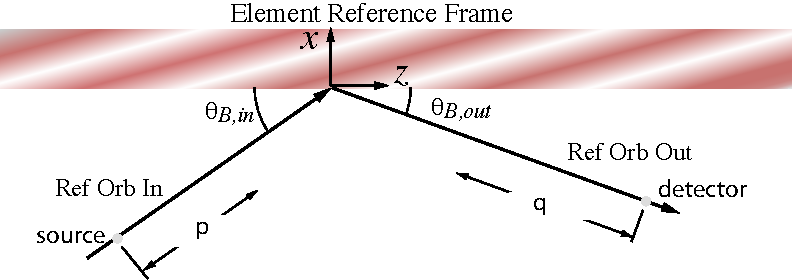
\includegraphics[width=5in]{surface-curvature.pdf}
  \caption[Surface curvature geometry.]
{Surface curvature geometry. The element reference frame used to describe surface curvature has the
$z$ axis pointing towards the interior of the element, and the $x$ axis in the plane defined by
the entrance and exit reference orbit.}
  \label{f:surface}
\end{figure}

%-----------------------------------------------------------------
\section{Surface Properties for X-Ray elements}
\label{s:s.curve}

The following X-ray elements have a surface which X-rays impinge upon:
\begin{example}
  crystal               \sref{s:crystal}
  detector              \sref{s:detector}
  diffraction_plate     \sref{s:diff.plate}
  mask                  \sref{s:mask}
  mirror, and           \sref{s:mirror}
  multilayer_mirror     \sref{s:multilayer}
  sample                \sref{s:sample}
\end{example}
[There is also the \vn{capillary} element but this element specifies
its surface differently.]

\index{spherical_curvature}\index{elliptical_curvature_x}
\index{elliptical_curvature_y}\index{elliptical_curvature_z}
The coordinate system used for characterizing the curvature of a surface is the element reference
frame as shown in \fig{f:surface}). This coordinate system has the $z$ axis pointing towards the
interior of the element, and the $x$ axis in the plane defined by the entrance and exit reference
orbit. In this coordinate system, the surface is an ellipsoid plus a fourth order polynomial in $x$
and $y$ plus a possible ``figure error'' contribution $z_\text{fig}$ defined by a surface grid:
\Begineq
  {-z} = \frac{1}{g_z} \, \left[ 1 - \sqrt{1 - \sign(g_x) \, (g_x \, x)^2 - \sign(g_y) \, (g_y \, y)^2} \right] + 
  \sum_{2 \le i+j \le 6} c_{ij} \, x^i \, y^j - z_\text{fig}
  \label{xs2ij4}
\Endeq
$z_\text{fig}$ is discussed in section~\sref{s:surf.grid} and is only present when the surface grid
\vn{type} is set to \vn{Figure_Error}.  In \Eq{xs2ij4} the $c_{ij}$ coefficients parameterize the fourth order
polynomial and $g_x, g_y$, and $g_z$ parameterize the ellipsoid with $\sign$ being the sign function
\Begineq
  \sign(g_i) \equiv \begin{cases} 1 & g_i > 0 \\ -1 & g_i < 0 \end{cases}
\Endeq
If $g_z$ is zero, the first term on the RHS of \Eq{xs2ij4} is ignored. If $g_x$, $g_y$, and $g_z$
are the same value $g$ then the ellipsoid is a sphere with radius $1/g$ The ellipsoid parameters are
set for an element by setting the element parameters
\begin{example}
  spherical_curvature    = <Real>
  elliptical_curvature_x = <Real>
  elliptical_curvature_y = <Real>
  elliptical_curvature_z = <Real>
\end{example}
and the correspondence between the ellipsoid parameters of \Eq{xs2ij4} and these parameters is:
\begin{example}
  \(g_x\) = elliptical_curvature_x + spherical_curvature
  \(g_y\) = elliptical_curvature_y + spherical_curvature
  \(g_z\) = elliptical_curvature_z + spherical_curvature
\end{example}
The polynomial coefficients $c_{ij}$ are set in the lattice file by setting the
element attributes
\index{surface curveture}
\begin{example}
  curvature_xM_yN = <Real>   
\end{example}
where \vn{M} and \vn{N} are integers in the range 0 through 6 with the restriction
\begin{example}
  2 \(\le\) M + N \(\le\) 6
\end{example}
Example:
\begin{example}
  c2: crystal, spherical_curvature = 1/4.7, curvature_x2_y0 = 0.37, ...
\end{example}
in this example, \vn{curvature_x2_y0} corresponds to the $c_{20}$ term
in \Eq{xs2ij4}. To get the effect of a nonzero $x^0\, y^0$, $x^1 \,
y^0$, or $x^0 \, y^1$ terms (since corresponding \vn{curvature_xN_yM}
are not permitted), element offsets and pitches can be used
(\sref{s:offset}).

Some useful formulas: Series expansion for a sphere of radius $R$:
\Begineq
  {-z} = \frac{x^2}{2 \, R} + \frac{x^4}{8 \, R^3} + \frac{x^6}{16 \, R^5} +
         \frac{y^2}{2 \, R} + \frac{y^4}{8 \, R^3} + \frac{y^6}{16 \, R^5} +
         \frac{x^2 \, y^2}{4 \, R^3} + \frac{3 \, x^4 \, y^2}{16 \, R^5} +
         \frac{3 \, x^2 \, y^4}{16 \, R^5} 
\Endeq
If $p$ is the distance from the source to the crystal, and $q$ is the
distance from the crystal to the detector, the radius of the Rowland
circle $R_s$ in the sagittal plane is given by\cite{b:del.rio}
\Begineq
  \frac{1}{p} + \frac{1}{q} = \frac{\sin\theta_{g,in} + \sin\theta_{g,out}}{R_s}
\Endeq
where $\theta_{g,in}$ and $\theta_{g,out}$ are the entrance and exit
graze angles. In the transverse plane (also called meridional plane),
the radius $R_t$ needed for foucusing is
\Begineq
  \frac{\sin^2\theta_{g,in}}{p} + \frac{\sin^2\theta_{g,out}}{q} = \frac{\sin\theta_{g,in} + \sin\theta_{g,out}}{R_t}
\Endeq

Example:
\begin{example}
  t_bragg = 1.3950647
  rt = 1  ! Crystal transverse radius
  rs = rt*(sin(t_bragg))^2
  c: crystal, crystal_type =  'Si(553)', b_param = -1,
        curvature_x0_y2 =  1 / (2 * rs), curvature_x0_y4 = 1 / (8 * rs^3),
        curvature_x2_y0 = 1 / (2 * rt), curvature_x4_y0 = 1 / (8 * rt^3),
\end{example}

%-----------------------------------------------------------------
\subsection{Surface Grid}
\label{s:surf.grid}
\index{surface grid}

A surface can be broken up into a grid of rectangles. This is useful,
for example, in breaking up a \vn{detector} element into pixel photo
receptors or in simulating a rough serface for \vn{crystal}s and other
elements. The general syntax is:
\begin{example}
  surface = \{
    grid = \{                
      type = <type_name>,                ! Off, Segmented, Figure_Error, or H_Misalign
      ix_bounds = (<ix_min>, <ix_max>),  ! Min/max index bounds in x-direction
      iy_bounds = (<iy_min>, <iy_max>),  ! Min/max index bounds in y-direction
      r0 = (<x0>, <y0>),                 ! (x,y) coordinates at grid origin
      dr = (<dx>, <dy>),                 ! width and height of pixels.
      ! Grid points used with type = H_Misalign:
      pt(<i>,<j>) = (<dz_dx>, <dz_dy>, <dz_dx_rms>, <dz_dy_rms>)
      ! Grid points used with type = Figure_Error:
      pt(<i>,<j>) = (<z>, <dz_dx>, <dz_dy>),    ! or
      pt(<i>,<j>) = <z>, 
                                         
          \} \}
\end{example}
Example:
\begin{example}
  ccd: crystal, surface = \{
          grid = \{
            type = h_misalign,
            r0 = (0.0, 0.01), dr = (0.005, 0.005),
            ix_bounds = (1, 57), iy_bounds = (-30, 10),
            pt(1,-30) = (0.001, -0.002, 0, 0), 
            pt(1,-29) = ..., 
          \} \}
\end{example}

The grid is a two dimensional with bounds given by the \vn{ix_bounds}
and \vn{iy_bounds} components. These two components must be present. In
the above example the grid is 57 pixels in $x$ and 41 pixels in $y$.

The physical placement of the grid on the element is determined by the
\vn{r0} and \vn{dr} components. \vn{r0} is optional and gives the
$(x,y)$ coordinates of the center of the pixel with index $(0,0)$. The
\vn{dr} component, which must be present, gives the pixal width and
height. Thus the center of the $(i,j)$ pixel is:
\begin{example}
  (x,y) = (r0(1), r0(2)) + (i*dr(1), j*dr(2))
\end{example}

There are several types of grids. What type of grid is determined by the \vn{type} component
Possible \vn{type} values are:
\begin{example}
  Figure_Error       ! Mesh defines the surface figure error.
  H_Misalign         ! Misalignment of crystal H vector
  Off                ! Ignore grid
  Segmented          ! Surface is a matrix of flat rectangles
\end{example}

\begin{description}
\item[Figure_Error] \Newline
With the \vn{type} parameter set to \vn{Figure_Error}, a figure error, $z_\text{fig}$ is added to
the surface curvature as shown in \Eq{xs2ij4}. $z_\text{fig}$ is determined by a spline
interpolation of the $z$ values of the grid of points defined by \vn{pt(<i>,<j>)}. For each point
\vn{pt(<i>,<j>)}, the $z$ value along with the $dz_dx$ and $dz_dy$ slopes can be specified or only
the $z$ value needs to be specified. With the later option the slopes will be computed by taking
finite differences of nearest neighbors.
%
\item[H_Misalign] \Newline
A setting of the \vn{type} attribute to \vn{H_Misalign} is used with crystals only. With
\vn{H_Misalign}, the grid defines misalignment of the $H$ vector which is the normal to the
diffracting planes of the crystal (\sref{s:crystal.tracking}).  When using \vn{H_Misalign}, each
\vn{pt(i,j)} component gives the misalignment of $H$ for the corresponding pixel. For an individual
photon, the misalignt of $H$ will be
\begin{example}
  dz_dx_tot = <dz_dx> + r1 * <dz_dx_rms>
  dz_dy_tot = <dz_dy> + r2 * <dz_dy_rms>
\end{example}
where \vn{dz_dx_tot} and \vn{dz_dy_tot} are the rotational misalignment (\sref{s:offset}) used
in the calculation, the quantities in brackets \vn{<...>} are components of \vn{pt}, and \vn{r1} and
\vn{r2} are Gaussian distributed random numbers with unit rms. These random numbers are regenerated
for each photon. Note: \vn{pt} is only used with \vn{H_Misalign}.
%
\item[Off] \Newline
When the \vn{type} component is set to \vn{Off}, the grid will not be used.
%
\item[Segmented] \Newline
When the \vn{type} component is set to \vn{Segmented}, the crystal surface is modeled as a grid of
flat ``rectangles'' (the actual shape is very close but not quite rectangular). Using a segmented
surface only makes sense when the surface is curved (see \Eq{xs2ij4}). There is one rectangle for
each pixel. Each rectangle has an extent in the $(x,y)$ transverse dimensions equal to the extent of
the corresponding pixel. \Eq{xs2ij4} is used to calculate the $z$ coordinate of the vertices of a given
rectangle and then these $z$ values are adjusted so that
\begin{example}
  1) The rectangle is flat (the verticies all lie on a plane).
  2) The rectangle contacts the unsegmented surface (\Eq{xs2ij4}) at two diagonally opposite vertices.
  3) The other two diagonaly opposite vertices will be as close as possible in the
     least squares sense from the unsegmented surface.
\end{example}
Note: The \vn{pt} component is not used here.
\end{description}

%-----------------------------------------------------------------
\section{Walls: Vacuum Chamber, Capillary and Mask}
\label{s:wall}
\index{wall}

The \vn{wall} attribute for an element is used to define:
\begin{example}
  vacuum chamber wall
  capillary element (\sref{s:capillary}) inside wall
  diffraction_plate (\sref{s:diff.plate}) geometry
\end{example}

The topics of the following subsections are:
\begin{example}
  \sref{s:wall.syntax}      General wall syntax.
  \sref{s:wall.section}      Cross-section construction. 
  \sref{s:wall.interpolation}      Capillary and vacuum chamber wall interpolation.
  \sref{s:wall.capillary}      Capillary wall.
  \sref{s:wall.vacuum}      Vacuum chamber wall.
  \sref{s:masking.wall}      Mask wall for diffraction_plate and mask elements.
\end{example}

%-----------------------------------------------------------------
\subsection{Wall Syntax}
\label{s:wall.syntax}

The syntax of the \vn{wall} attribute is:
\begin{example}
  wall = \{
    superimpose = <T/F>,               ! Chamber wall only
    thickness = <real>                 ! Default thickness. 
    opaque_material = <material_type>  ! Default opaque material. 
    clear_material = <material_type>   ! Default clear material. 
    section = \{ 
      type = <section_type>,           ! Chamber Mask, and Diffraction_plate only
      s = <longitudinal_position>,     ! Relative to beginning of element.
      r0 = (<x0>, <y0>),               ! section (x,y) origin
      absolute_vertices = <T/F>,       ! Vertex nums: abs or relative to r0? Default = F.
      material = <material_type>,      ! Mask and Diffraction_plate only.
      thickness = <real>,              ! Mask and Diffraction_plate only.
      dr_ds = <value>,                 ! Capillary and Chamber only
      v(1) = \{<x>, <y>, <radius_x>, <radius_y>, <tilt>\}, 
      v(2) = \{ ... \},
      ...\},
    section = \{
      s = <longitudinal_position>, 
      v(1) = \{... \},
      ... \},
    ... \}
\end{example}
A \vn{wall} begins with ``\vn{wall = \{}'' and ends with a
``\vn{\}}''. In between are a number of individual cross-section
structures. Each individual cross-section begins with ``\vn{section =
\{}'' and ends with a ``\vn{\}}''. The \vn{s} parameter of a
cross-section gives the longitudinal position of the cross-section.
Example:
\begin{example}
  this_cap: capillary, 
    wall = \{   
      section = \{ ! cross-section with top/bottom symmetry
        s = 0, v(1) =  \{0.02, 0.00\}, 
        v(2) = \{0.00, 0.02, 0.02\}, v(3) = \{-0.01, 0.01\} \}, 
      section = \{  ! Cross-section that is a tilted ellipse.
        s = 0.34, 
        v(1) = \{0.003, -0.001, 0.015, 0.008, 0.2*pi\} \} \}
\end{example}
In this example an element called \vn{this_cap} is a \vn{capillary}
whose wall is defined by two cross-sections.

%------------------

\begin{figure}[tb]
  \centering
  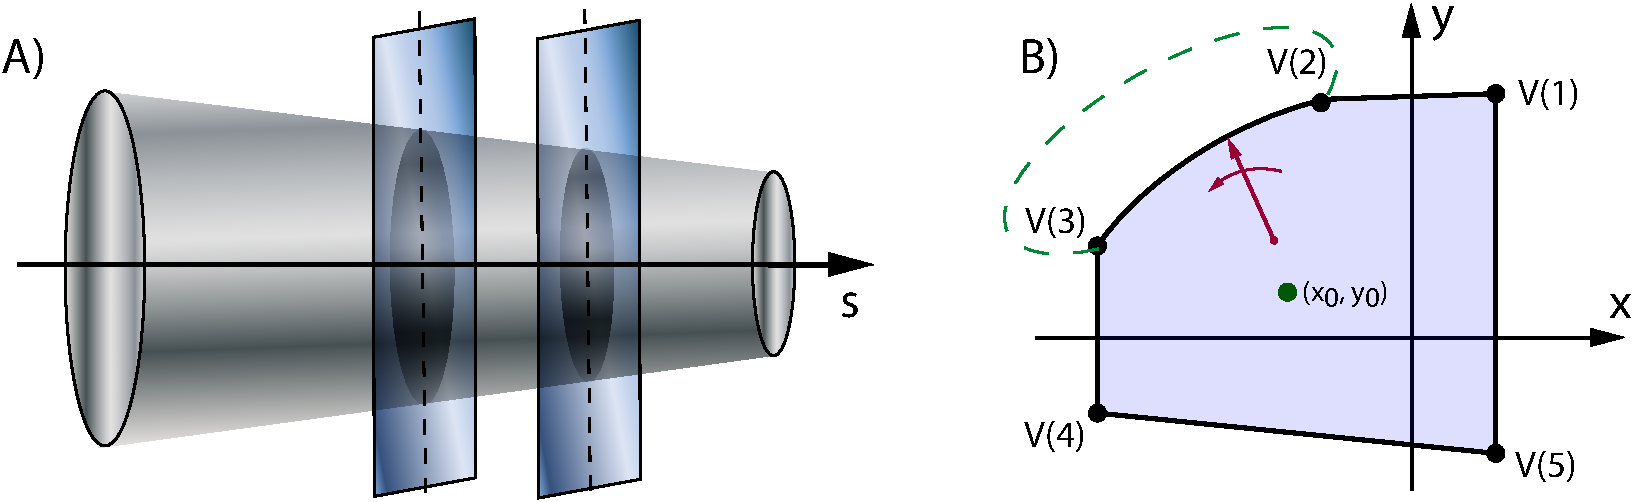
\includegraphics[width=6in]{chamber-wall.pdf}
  \caption[Capillary or vacuum chamber wall.]
{A) The inside wall of a capillary or the vacuum chamber wall of a
non-capillary element is defined by a number of cross-sectional
slices.  B) Each cross-section is made up of a number of vertices. The
segments between the vertices can be either a line segment, the arc of
a circle, or a section of an ellipse.}
  \label{f:chamber.wall}
\end{figure}

%-----------------------------------------------------------------
\subsection{Wall Sections}
\label{s:wall.section}

The wall is defined by a number of cross-sectional slices. For
\fig{f:chamber.wall}A shows the geometry for \vn{capillary} or vacuum
chamber walls.  Each cross-section is defined by a longitudinal
position $s$ relative to the beginning of the element and a number of
vertices. The verticies are defined with respect to the local sector
origin $r_0$ except if \vn{absolute_vertices} is set to \vn{True} in
which case the vertex numbers are taken as absolute. The arc between
each vertex may be either a straight line, an arc of a circle, or a
section of an ellipse. For a capillary it is mandatory that a
cross-section be convex. That is, given any two points within the
cross-section, all points on the line segment connecting them must be
within the cross-section.

The \vn{v(<j>)} within a cross-section define the vertices for each
cross-section. The vertices are defined with respect to the section
origin given by \vn{r0}. Each \vn{v(<j>)} has five
parameters. It is mandatory to specify the first two parameters
\vn{<x>} and \vn{<y>}. Specifying the rest, \vn{<radius_x>},
\vn{<radius_y>}, and \vn{<tilt>}, is optional. The default values, if
not specified, is zero. The point (\vn{<x>}, \vn{<y>}) defines the
position of the vertex. The parameters \vn{<radius_x>},
\vn{<radius_y>}, and \vn{<tilt>} define the shape of the segment of
the cross-section between the given vertex and the preceding one.
\begin{example}
  <radius_x>  = 0, <radius_y>  = 0   --> Straight line segment.
  <radius_x> != 0, <radius_y>  = 0   --> Circular arc with radius = radius_x
  <radius_x>  = 0, <radius_y> != 0   --> Illegal!
  <radius_x> != 0, <radius_y> != 0   --> Ellipse section.
\end{example}
When an ellipse is specified, \vn{<radius_x>}, and \vn{<radius_y>} are
the half width and half height of the semi-major axes and the
\vn{<tilt>} parameter gives the tilt of the ellipse. \vn{<radius_x>}
and \vn{<radius_y>} must not be negative.

In the example above, for the first cross-section, \vn{v(2)}
specifies a non-zero \vn{<radius_x>} and, by default, \vn{<radius_y>}
is zero. Thus the segment of the cross-section between \vn{v(1)} and
\vn{v(2)} is circular in nature with a radius of 0.02. Since \vn{v(3)}
does not specify \vn{<radius_x>} nor \vn{<radius_y>}, the
cross-section between \vn{v(2)} and \vn{v(3)} is a straight line
segment.

The vertex points must be arranged in a ``counter clockwise manner''. 
For vertices \vn{<v(i)>} and \vn{<v(i+1)>} connected by a line segment
this translates to
\Begineq
  0 < \theta_{i+1} - \theta_{i} \pmod{2\pi} < \pi
\Endeq
where $(r_n, \theta_n)$ are the polar coordinates of the $n^{th}$
vertex. For vertices connected by an arc, ``counter clockwise manner''
means that the line segment with one end at the center of the arc and
the other end traversing the arc from \vn{<v(i)>} to \vn{<v(i+1)>}
rotates in counter clockwise as shown in
\fig{f:chamber.wall}B. 

The red line segment with one end at the center of the arc and the
other end traversing the arc from, in this case, $V(2)$ to $V(3)$,
rotates in counter clockwise manner. In general, there are two
solutions for constructing such an arc. For positive radii, the
solution chosen is the one whose center is closest to the section
origin $(x_0, y_0)$. If the radii are negative, the center point will
be the point farthest from the origin (the dashed line between $V(2)$
and $V(3)$ in the figure).

A restriction on cross-sections is that the section origin $(x_0,
y_0)$ must be in the interior of any cross-section and that for any
cross-section a line drawn from the origin at any given angle $\theta$
will intersect the cross-section at exactly one point as shown in
\fig{f:chamber.wall}B. This is an important point in the construction
of the wall between cross-sections as explained below.

The last vertex specified, call it \vn{<v(n)>}, should not have the
same \vn{<x>}, \vn{<y>} values as the first vertex \vn{<v(1)>}. That
is, there will be a segment of the cross-section connecting
\vn{<v(n)>} to \vn{<v(1)>}. The geometry of this segment is determined
by the parameters of \vn{<v(1)>}.

If there is mirror symmetry about the $x$ or $y$ axis for a
cross-section, the ``mirrored'' vertices, on the ``negative'' side of
the mirror plane, do not have to be specified. Thus if all the vertex
points of a cross-section are in the first quadrant, that is, all
\vn{<x>} and \vn{<y>} are zero or positive, mirror symmetry about both
the $x$ and $y$ axes is assumed. If all the \vn{<y>} values are zero
or positive and some \vn{<x>} values are positive and some are
negative, mirror symmetry about the $x$ axis is assumed. Finally, if
all the \vn{<x>} values are zero or positive but some \vn{<y>} values
are positive and some are negative, symmetry about the $y$ axis is
assumed. For example, for the first in the above example, since all
the \vn{<y>} values are non-negative and there are positive and
negative \vn{<x>} values, symmetry about the $x$ axis is assumed.

The one exception to the above rule that (\vn{<x>}, \vn{<y>}) is the
vertex center is when a single vertex \vn{v(1)} is specified for a
cross-section with a non-zero \vn{<radius_x>}. In this case,
(\vn{<x>}, \vn{<y>}) are taken to be the center of the circle or
ellipse. For example, if a single vertex is specified for a
cross-section as:
\begin{example}
  section = \{s = 0.3, v(1) = \{0.03, -0.01, 0.15, 0.08, 0.2\}\}
\end{example}
the cross-section will be an ellipse with center at $(0.03, -0.01)$
with a tilt of $0.2$ and axes radii of $0.15$ and $0.08$. If
a cross-section has a single vertex and \vn{<radius_x>} is not
specified, the cross-section is a rectangle. For example
\begin{example}
  section = \{s = 0.3, v(1) = \{0.03, 0.01\}\}
\end{example}

%-----------------------------------------------------------------
\subsection{Interpolation Between Sections}
\label{s:wall.interpolation}

\begin{figure}[tb]
  \centering
  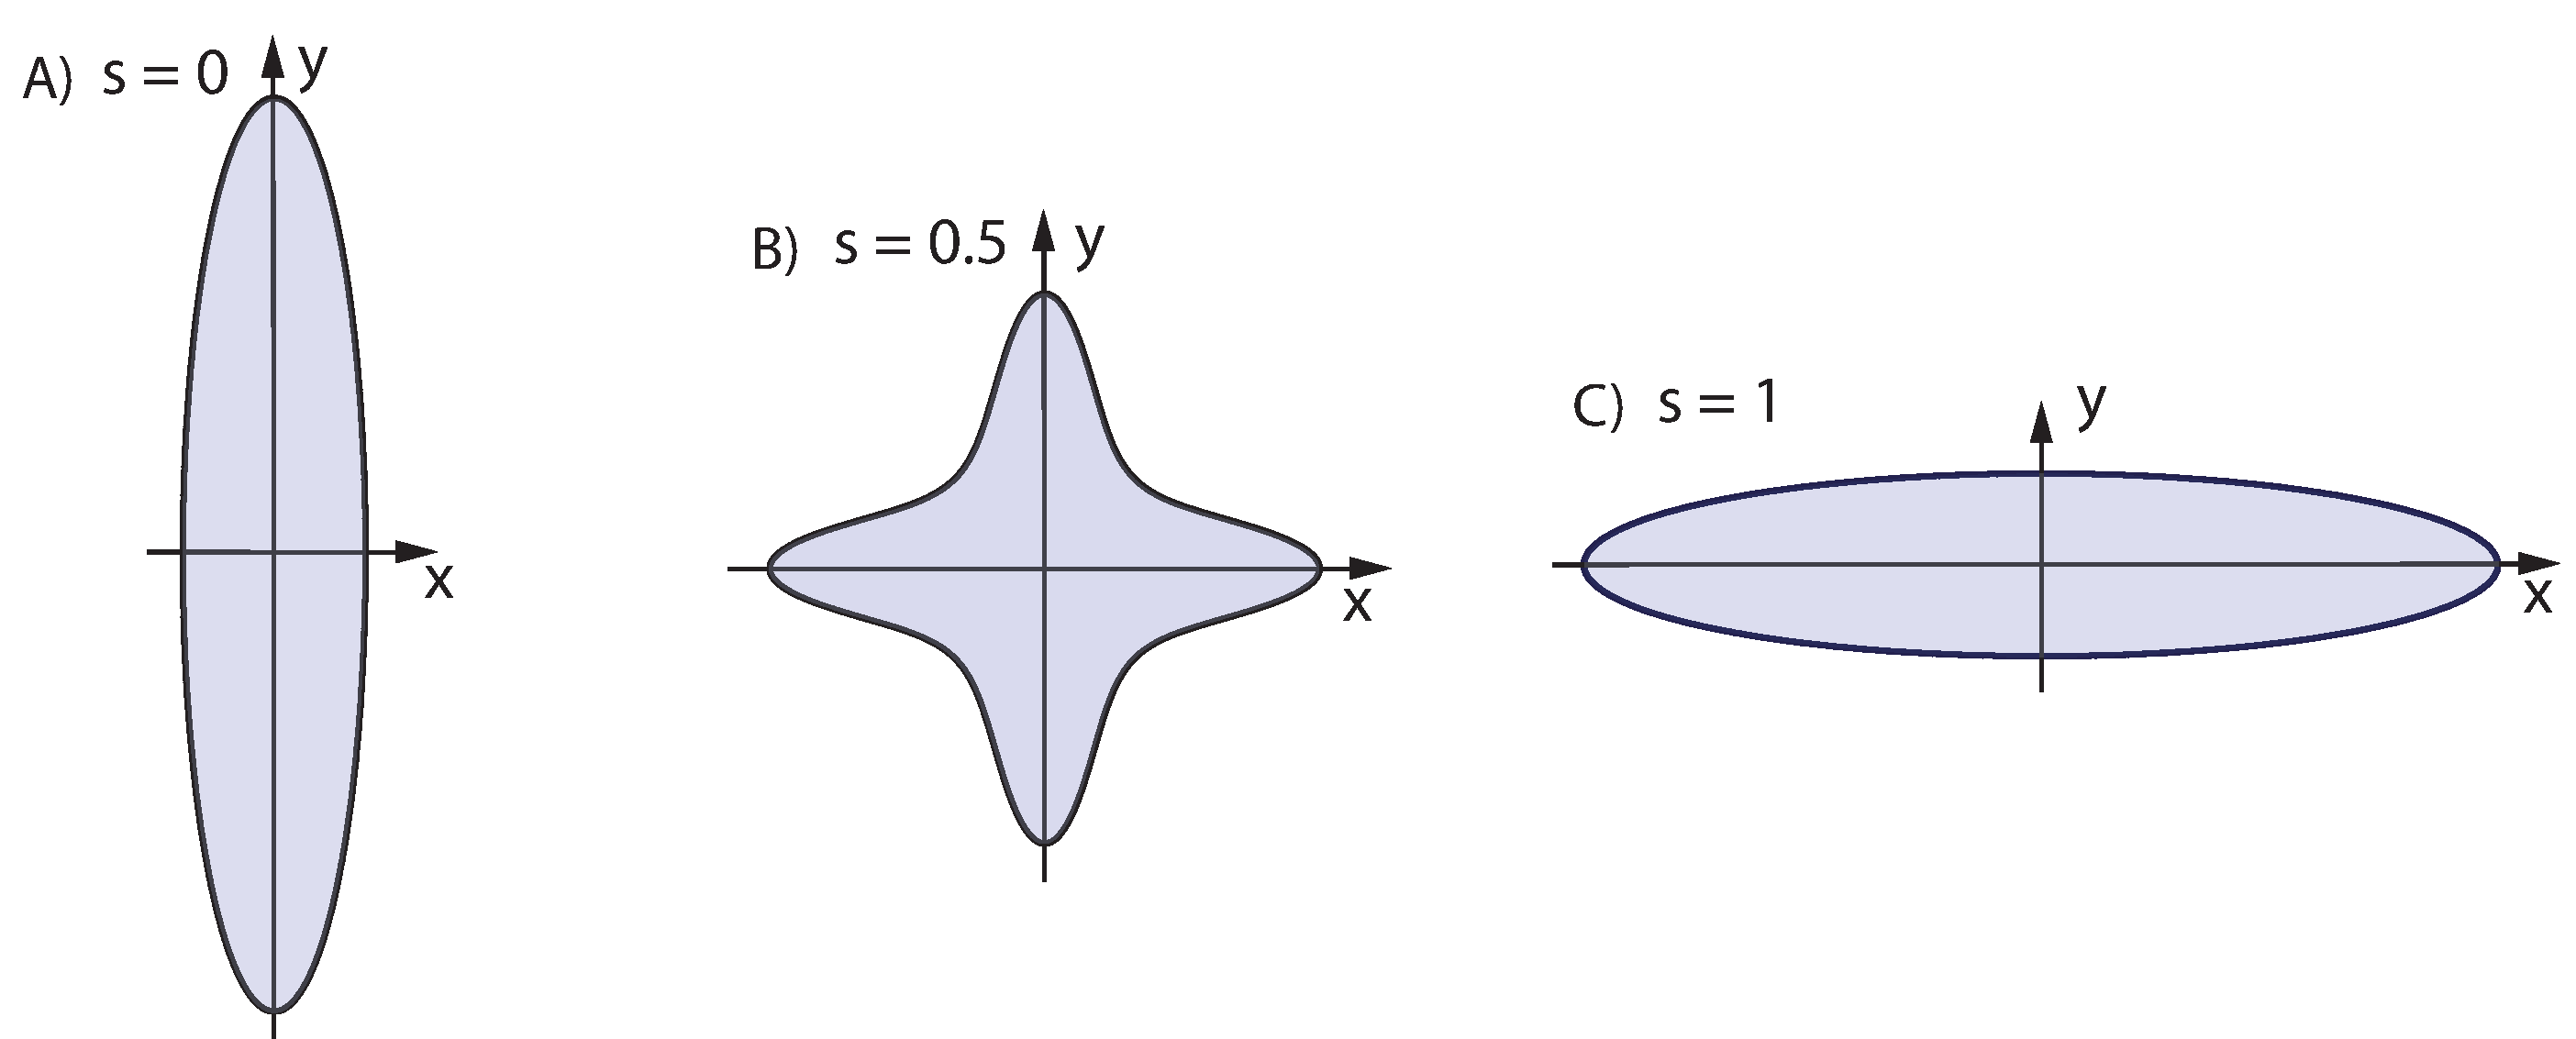
\includegraphics[width=4in]{concave-capillary.pdf}
  \caption[Convex cross-sections do not guarantee a convex volume.]
{Example where convex cross-sections do not produce a convex volume.
Cross-sections (A) and (C) are ellipses with a 5 to 1 aspect ratio.
Half way in between, linear interpolation produces a convex cross-section
as shown in (B).} 
  \label{f:concave.capillary}
\end{figure}

For \vn{capillary} and vacuum chamber walls, the wall between
cross-sections, is defined by interpolation. At a given $s$ position,
the $r, \theta$ coordinate system in the transverse $x, y$ plane is
defined with respect to an origin $\bfr_O(s)$ given by a linear
interpolaion of the origins of the cross-sections to either side of the
given $s$ position. Let $s_1$ denote the position of the cross-section
just before $s$ and $s_2$ denote the position of the cross-section
just after $s$. Let $\bfr_{01}$ be the $(x_0, y_0)$ origin defined
for the cross section at $s_1$ and $\bfr_{02}$ be the $(x_0, y_0)$
origin defined for the cross section at $s_2$. Then
\Begineq
  \bfr_O(s) = (1 - \stilde) \, \bfr_{01} + \stilde \, \bfr_{02}
\Endeq
where 
\Begineq
  \stilde \equiv \frac{s - s_1}{s_2 - s_1}
\Endeq

Let $r_{c1}(\theta)$ and $r_{c2}(\theta)$ be the radiusus of the wall
as a function of $\theta$ for the cross-sections at $s = s_1$ and $s =
s_2$ respectively. The wall $r_c(\theta, s)$ at any point $s$ between
$s_1$ and $s_2$ is then defined by the equation
\Begineq
  r_c(\theta, s) = p_1(\stilde) \, r_{c1}(\theta) + p_2(\stilde) \, r_{c2}(\theta)
\Endeq
where $p_1$ and $p_2$ are cubic polynomials parameterized by
\begin{align}
  p_1 &= 1 - \stilde + a_1 \, \stilde + a_2 \, \stilde^2 + a_3 \, \stilde^3 \CRNO
  p_2 &= \stilde + b_1 \, \stilde + b_2 \, \stilde^2 + b_3 \, \stilde^3 
\end{align}
If $a_i = b_i = 0$ for all $i = 1, 2, 3$, the interpolation is linear
and this is the default if either of the parameters \vn{dr_ds1} and
\vn{dr_ds2} are not given in the wall definition. These parameters are
the slopes of the wall with respect to $s$ at the end points
\begin{equation}
  \text{dr_ds1} \equiv \left. \frac{d\overline{r}}{ds} \right|_{s = s_1} \comma \qquad
  \text{dr_ds2} \equiv \left. \frac{d\overline{r}}{ds} \right|_{s = s_2} 
\end{equation}
where $\overline{r}$ is the average $r$ averaged over all
$\theta$. When {\em both} \vn{dr_ds1} and \vn{dr_ds2} are specified, the $a_i$
and $b_i$ are calculated so that the slopes of the wall match 
the values of \vn{dr_ds1} and \vn{dr_ds2} along with the constraints.
\begin{align}
  p_1(0) &= 1 \comma \qquad p_1(1) = 0 \CRNO
  p_2(0) &= 0 \comma \qquad p_2(1) = 1 \\
  M &\equiv a_1^2 + a_2^2 + a_3^2 + b_1^2 + b_2^2 + b_3^2 \text{ is a minimum}
  \nonumber
\end{align}
The last constraint ensures a ``smooth'' transition between the two cross-sections.

To refer to a cross-section parameters after an element has been
defined, the following syntax is used:
\begin{example}
  ele_name[wall%section(n)%v(j)%x]   ! x value of j^th vertex of n^th cross-section
\end{example}

%-----------------------------------------------------------------
\subsection{Capillary Wall}
\label{s:wall.capillary}
\index{capillary!wall}

For a \vn{capillary}, \vn{s} must be zero for the first cross-section and
the length of the capillary is given by the value of \vn{s} of the
last cross-section.

For a \vn{capillary}, in order for \bmad to quickly track photons,
\bmad assumes that the volume between the cross-sections is
convex. The volume will be convex if each cross-section $r_c(\theta,
s)$ at any given $s$ is convex. Note that it is {\em not} sufficient
for $r_c(\theta, s)$ to be convex at the specified cross-sections as
shown in \fig{f:concave.capillary}. Also note that it is perfectly
fine for the total capillary volume to not be convex.

%-----------------------------------------------------------------
\subsection{Vacuum Chamber Wall}
\label{s:wall.vacuum}

The vacuum chamber wall is independent of the element apertures
(\sref{s:limit}). Unless a program is specifically constructed, the
presence of a vacuum chamber wall will not affect particle tracking.

The vacuum chamber wall defined for an element may be shorter or
longer than the element.  The vacuum chamber wall for a particular
lattice branch is the sum of all the chamber walls of the individual
elements. That is, the chamber wall at any given point is determined
by interpolation of the nearest sections upstream and downstream to
the point.  Thus a given lattice element need not contain a \vn{wall}
component for the chamber wall to be well defined at the element. 

The exception to the above rule is when a \vn{section} has its
\vn{type} component set to either:
\begin{example}
  wall_start
  wall_end
\end{example}
\vn{wall_start} and \vn{wall_end} sections must come in pairs. The
next section after a \vn{wall_end} section (if this section is not
the last section in the lattice) must be a \vn{wall_start} section.
If a section has a \vn{type} of \vn{wall_start}, the region between
that section and the previous section (which must be a \vn{wall_end}
section) will be considered to have no wall. If the \vn{wall_start}
section is the first section of the lattice branch, the region of no
wall will start at the beginning of the branch. Similarly, if a
section has a \vn{type} of \vn{wall_end}, the region between that
section and the next section (or the end of the lattice branch if
there is no next seciton) will not have a wall.

The chamber walls of any two elements may not overlap. The exception
is when the \vn{superimpose} attribute for a wall of an element is set
to True. In this case, any other wall cross-sections from any other
elements that overlap the superimposed wall are discarded.
Superposition of a wall is useful, for example, in introducing mask
regions into the wall.

If a branch has a closed geometry (\sref{s:param}), wall sections that
extend beyound the ends of the branch are ``wrapped'' around.

If a particle is past the last wall cross-section or before the first
wall cross-section, The following rules are used: If the branch has a
\vn{closed geometry}, the wall will be interpolated between the last
and first cross-sections. If the branch has an \vn{open} geometry, the
wall is taken to have a constant cross-section in these regions. 

The chamber wall is defined with respect to the local coordinate
system (\sref{s:ref}). That is, in a bend a wall that has a constant
cross section is a section of a torus.

\index{patch!and chamber wall}
\vn{Patch} elements (\sref{s:patch}) complicate the wall geometry
since the coordinate system at the end of the \vn{patch} may be
arbitrarily located relative to the beginning of the patch. To avoid
confusion as to what coordinate system a wall section belongs to,
\vn{patch} elements are not allowed to define a wall. The wall through
a patch is determined by the closest wall sections of neighboring
elements.

%-------------------

\begin{figure}[tb]
  \centering
  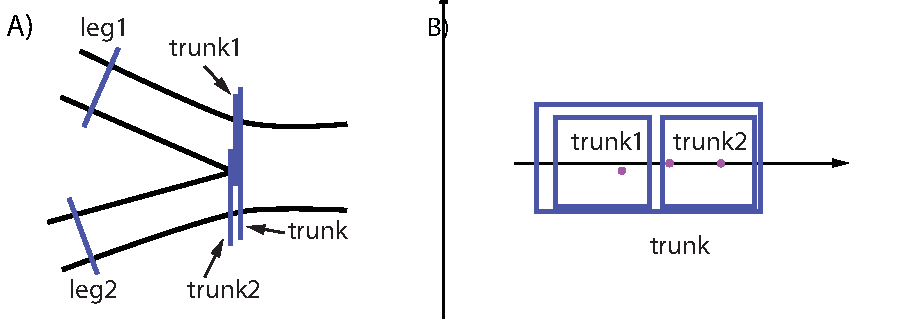
\includegraphics[width=6in]{crotch.pdf}
  \caption[vacuum chamber crotch geometry.]
{A) Crotch geometry: Two pipes labeled ``leg1'' and ``leg2'' merge
into a single pipe called the ``trunk'' pipe. Five wall sections are
used to define the crotch geometry (solid lines). Dashed lines
represent sections not involved in defining the crotch. For purposes
of illustration, the three trunk sections are displaced longitudinally
but in reality must have the same longitudinal coordinate.  B) Example
layout of the trunk1, trunk2 and trunk wall sections. $O_1$, $O_2$
and $O$ are the $x_0, y_0$ origins of the sections.}
  \label{f:crotch}
\end{figure}

%-------------------

\index{crotch chamber geometry}
Each section has a \vn{type} attribute. This attribute is not used for 
\vn{capillary} elements. For a vacuum chamber wall, the \vn{type} 
attribute is used to dscribe a ``crotch'' geometry where
two pipes merge into one pipe. The possible values for the \vn{type} 
attribute are:
\begin{example}
  normal     ! default
  leg1
  leg2
  trunk1
  trunk2
  trunk
\end{example}
The geometry of a crotch is shown in \fig{f:crotch}A. Two pipes,
called ``leg1'' and ``leg2'', merge into one pipe called the ``trunk''
pipe.  The trunk pipe can be either upstream or downstream of the leg
pipes.  To describe this situation, five sections are needed: One
section in each leg pipe which need to have their \vn{type} attribute
set to \vn{leg1} and \vn{leg2}, and three sections in the trunk with
one having a a \vn{type} attribute of \vn{trunk1}, another having a
\vn{type} attribute of \vn{trunk2} and the third haveing a \vn{type}
attribute of \vn{trunk}. There can be no sections between the leg
sections and the trunk sections.

All three trunk sections must be associated with the same element and
have the same \vn{s} value. In the list of sections of the element
containing the trunk elements, the \vn{trunk1} and \vn{trunk2}
sections must be listed first if the leg pipes are upstream of the
trunk pipe (the situation shown in the figure) and must be listed last
if the leg pipes are downstream. That is, the \vn{trunk1} and
\vn{trunk2} sections are ``between'' the leg sections and the
\vn{trunk} section. It does not matter if \vn{trunk1} is before or
after \vn{trunk2}.

The \vn{trunk1} and \vn{trunk2} sections must not overlap and the
\vn{trunk} section must be constructed so that its area is the union
of the areas of \vn{trunk1} and \vn{trunk2}. An example is illustrated
in \fig{f:crotch}B. Here the \vn{trunk1} and \vn{trunk2} sections are
squares with origins labeled $O_1$ and $O_2$ in the figure. By
necessity, these origins must be different since each must lie within
the boundaries of their respective areas. The \vn{trunk} section is a
rectagle encomposing the two squares and has an origin labeled $O$.

Between \vn{leg1} and \vn{trunk1} sections the wall is interpolated
using these two section. Similarly for the region between \vn{leg2}
and \vn{trunk2} sections. Away from these regions interpolation is
done as outlined in \sref{s:wall.interpolation}. However, these two
regions need a different interpolation scheme since, \vn{leg1} and
\vn{trunk1}, as well as \vn{leg2} and \vn{trunk2} sections do not have
to be parallel to each other.

%-----------------------------------------------------------------
\subsection{Mask Wall For Diffraction Plate and Mask Elements}
\label{s:masking.wall}

\begin{figure}[tb]
  \centering
  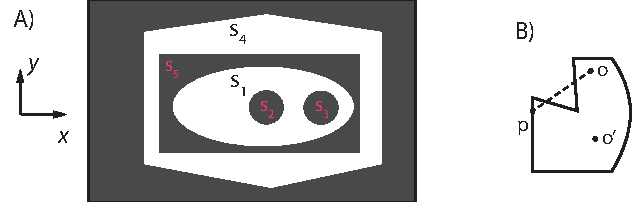
\includegraphics[width=5in]{diffraction-plate.pdf}
  \caption[Example mask wall]{
A) The diffraction plate or mask surface is divided into ``clear'' (white) and
``opaque'' (black) areas. In this example there are two clear sections
labeled \#1 and \#2. B) All wall sections must be star shaped with
respect to the section's origin. In this example, The section is {\em
not} star shaped since a line drawn from the origin point $o$ to the
point $p$ on the boundary intersects the boundary twice in between. In
this case the section can be made star shaped by moving the origin to
$o'$.
  }
  \label{f:diff.plate}
\end{figure}

The \vn{wall} of a \vn{diffraction_plate} or \vn{mask} element
specifies what areas of the
element will transmit or reflect particle and what areas will not. The
areas where there is transmission or reflection are called ``clear''
areas and everything else is called ``opaque''. 

A \vn{wall} is comprised a a ordered list of \vn{sections} as
discussed in \sref{s:wall.section}. Each section of the wall must have
its \vn{type} attribute set to one of:
\begin{example}
  clear
  opaque
\end{example}
A section is called ``clear'' or ``opaque'' depending upon the setting
of its \vn{type} attribute. Do not confuse ``clear section'' with 
``clear area''.

A clear area is defined by one or more consecutive wall sections. The
first section that defines a clear area must be a clear section.  All
the other sections associated with a clear area must be opaque sections.
That is, a clear area starts with a clear section and any preceeding
opaque sections up to the next clear section or the end of the section
list. As a consequence of the above rules, the fist section of the
wall must be a clear section and the number of clear areas is equal to
the number of clear sections.

The default behavior is that a photon will be transmitted if it is
within any clear area. A photon is considered to be within a given
clear area if its $(x,y)$ coordinates put in within the corresponding
clear section but not within any \vn{opaque} section of the clear area.
\vn{Opaque} sections only affect the clear area they are associated
with. See the example below.

Any clear section can be given a \vn{material} and
\vn{thickness}. Available materials are listed in
\sref{s:cryst.list}. A photon transversing a clear area with a defined
material will be attenuated and have a phase shift. Note that
\vn{material} and \vn{thickness} properties are not to be assigned to
\vn{opaque} sections.

To enable \bmad to quickly calculate whether a photon has landed on a
clear or opaque section, All sections, both clear and opaque, must be
``star shaped'' with respect to the $(x_0, y_0)$ origin used by the
section. That is, a line drawn from the section origin to any point on
the section boundary must not pass through any boundary points of the
section in between. This is illustrated in \fig{f:diff.plate}B where
the section is not star shaped since a line drawn from the origin $o$
to the point $p$ on the boundary passes through two boundary points in
between. In this case the section can trivially be made star shaped by
moving the origin to point $o'$. If it is not possible to make a
section star shaped by moving the origin, the section must be divided
into multiple sections.

An example geometry is shown in \fig{f:diff.plate}A.
In the figure, there are two openings labeled \#1, and \#2. A
wall that constructs this geometry is:
\begin{example}
  z_plate: diffraction_plate, wall = \{
    thickness = <real>
    opaque_material = <material_type>
    clear_material = <material_type>
    section = \{           ! Clear area \# 1
      type = clear, 
      v(1) = \{0.04, 0\}, v(2) = \{0.04, 0.022\},
      v(3) = \{0, 0.03\},
    section = \{
      type = opaque,
      v(1) = \{0.032, 0.016\},
    section = \{          ! Clear area \# 2
      type = clear,
      v(1) = \{0, 0, 0.03, 0.013\},
    section = \{
      type = opaque,
      v(1) = \{0, 0, 0.005\},
    section = \{
      type = opaque,
      r0 = (0.02, 0.00),
      v(1) = \{0, 0, 0.005\} \}
\end{example}
Clear area \#1 has a clear section and one opaque section. These
sections rely on the four fold symmetry of the sections so that only
points in the first quadrant need be specified. Clear area \#2 has one
clear section in the shape of an ellipse with two opaque circles. Notice
that the \vn{opaque} section of clear area \#1 does not affect the clear
area \#2 even though it (completely) overlaps clear area \#2.

Sections may overlap and a opaque section does not have to be wholly
within the corresponding clear section. If a photon is within multiple
clear areas then, for the purposes of calculation, it is considered to
be within the first possible clear area in the list.

%-----------------------------------------------------------------
\section{Length Attributes}
\label{s:l}

\index{length of elements}
\index{l|hyperbf}
\index{l_chord|hyperbf}
\index{rbend}
\index{sbend}
The length attributes are
\begin{example}
  l       = <Real>  ! 
  l_chord = <Real>  ! Chord length of a bend. Dependent attribute.
\end{example}
The length \vn{l} is the path length of the reference particle. The
one exception is for an \vn{rbend}, the length \vn{l} set in the
lattice file is the chord length (\sref{s:bend}). internally, \bmad
converts all \vn{rbend}s to \vn{sbend}s and stores the chord length
under the \vn{l_chord} attribute.
Example:
\begin{example}
  b: rbend, l = 0.6   ! For rbends, l will be converted to l_chord
\end{example}

\index{girder}
For a \vn{girder} element the length \vn{l} is a dependent attribute
and is set by \bmad to be the difference in longitudinal position $s$
of the downstream end of the last element supported relative to the
upstream end of the first element. 

\index{wiggler}
For \vn{wiggler}s, the length \vn{l} is not the same as the
path length for a particle with the reference energy starting on the
reference orbit. See~\sref{s:ref}.

\index{patch}
For \vn{patch} elements the \vn{l} length is, by definition, equal to
\vn{z_offset}. For \vn{patch} elements, \vn{l} is a dependent
attribute and will be automatically set to \vn{z_offset} by \bmad.

\index{capillary}
The length of a \vn{capillary} element is a dependent variable and is
given by the value of \vn{s} of the last wall cross-section
(\sref{s:wall.capillary}).

\index{crystal}
The length of a crystal is zero for Bragg diffraction and is a
dependent attribute dependent upon the crystal thickness for Laue
diffraction. See \sref{s:crystal} for more details.

%-----------------------------------------------------------------
\section{Is_on Attribute}
\label{s:is.on}
\index{is_on|hyperbf}

The \vn{is_on} attribute
\begin{example}
  is_on = <Logical>
\end{example}
is used to turn an element off. Turning
an element off essentially converts it into a drift.
Example
\begin{example}
  q1: quad, l = 0.6, k1 = 0.95
  q1[is_on] = False
\end{example}

\index{aperture}
\index{reference orbit}
\index{reference energy}
\vn{is_on} does not affect any apertures that are set. Additionally,
\vn{is_on} does not affect the reference orbit. Therefore, turning 
off an \vn{lcavity} will not affect the reference energy.

The following elements cannot be ``turned off:''
\begin{example}
  beginning_ele
  capillary
  crystal
  drift
  fiducial
  floor_shift
  patch
  group
  null_ele
  overlay
  hybrid
  mirror
  multilayer_mirror
  photon_init
  sample
\end{example}


%-----------------------------------------------------------------
\section{Multipole Attributes: Magnetic and Electric}
\label{s:multip}

Multipole formulas for are given in \sref{s:mag.field} and \sref{s:elec.field}. Note that
the setting of \vn{field_master} (\sref{s:field.master}) will determine if multipoles
are interpreted as normalized or unnormalized.

\index{multipole!knl, tn|hyperbf} 
\index{multipole}
A \vn{multipole} (\sref{s:mult}) element specifies its magnetic
multipole components using an Amplitude (\vn{KnL}) and a tilt
(\vn{Tn})
\begin{example}
  KnL = <Real>
  Tn  = <Real>  ! Default is $pi$/(2n + 2)
\end{example}
Where \vn{n} is an integer in the range from 0 (dipole component)
through 21.  If \vn{Tn} is given without a value, a default of
$pi$/(2n + 2) will be used producing a skew field. Example:
\begin{example}
  m: multipole, k1l = 0.32, t1  ! Skew quadrupole of strength 0.32
\end{example}
Following \vn{MAD}, a non-zero dipole (\vn{K0L} component will affect
the reference orbit (just like a normal dipole will). This is not true
for any other element.

\index{ab_multipole}
\index{multipole!an, bn|hyperbf} 
An \vn{ab_multipole} (\sref{s:ab.m}) specifies magnetic multipoles
using normal (\vn{Bn}) and skew (\vn{An}) components:
\begin{example}
  An = <Real>
  Bn = <Real>
\end{example}
Here \vn{n} ranges from 0 (dipole component) through 21. Example:
\begin{example}
  q1: ab_multipole, b2 = 0.12, a20 = 1e7, field_master = T
\end{example}

\index{r0_mag}\index{scale_multipoles}
Elements like \vn{quadrupoles} and \vn{sextupoles} can have assigned to them both magnetic and
electric multipole fields. In this case, the magnetic fields are specified using the same convention
as the \vn{ab_multipole}.  For such non-multipole elements, the magnetic multipole strength is
scaled by a factor $F \, r_0^{n_\text{ref}} / r_0^n$ (cf.~\Eq{ababf}) where $F$ is the strength of
the element (for example $F$ is $K1 \cdot L$ for a quadrupole), and $r_0$ is the ``measurement
radius'' and is set by the \vn{r0_mag} attribute. The default value of $r_0$.  This behavior may be
turned off by setting the \vn{scale_multipoles} attribute.  Example:
\begin{example}
  q1: quadrupole, b2 = 0.12, a20 = 1e7, scale_multipoles = F
\end{example}
Alternatively, a value of zero (the default) for \vn{r0_mag} is equivalent to setting
\vn{scale_multipoles} to False.

Electric multipoles are specified using normal (\vn{Bn_elec}) and skew
(\vn{An_elec}) components. \begin{example}
  An_elec = <Real>
  Bn_elec = <Real>
\end{example}
Here \vn{n} ranges from 0 (dipole component) through 21. Like the magnetic multipoles, 
a measurement radius \vn{r0_elec} can be used to scale the multipoles as explained in 
\sref{s:elec.field}.
Example:
\begin{example}
  q1: quadrupole, l = 1.2, b2_elec = 1e6, r0_elec = 0.034
\end{example}
See \sref{s:elec.field} for how electric multipoles are defined. Notice that Electric
multipoles are never scalled by the element's field strength as they are with magnetic
multipoles. If the value of \vn{r0_elec} is zero (the default) the multipoles will not
be scalled. 

Unlike magnetic multipoles, there are no factors of the reference momentum nor the element
length in the definition for electric multipoles. That is, electric multipole values
represent the field and not the normalized integrated field. Thus an electric multipole
associated with a zero length element will have no effect on tracking. This being the
case, \bmad does not allow electric multipole values to be specified for \vn{multipole}
and \vn{ab_multipole} elements. Indeed, in the limit of zero element length at constant
integrated electric field strength, the equations of motion are singular since, unlike the
magnetic case, the infinite fringe fields give rise to infinite energy shifts.

\index{multipoles_on}
The magnetic and electric multipole kick can be toggled on or off using the
\vn{multipoles_on} attribute. Example:
\begin{example}
  call, file = 'lattice.bmad'             ! Read in a lattice file
  quadrupole::*[multipoles_on] = False    ! But I want the multipoles off.
  q1[k1] = 0.3                            ! k1 attribute not affected.
\end{example}
\vn{multipoles_on} only effect multipoles specified by \vn{An}, \vn{Bn}, \vn{An_elec}, or
\vn{Bn_elec}. Other multipoles, like the \vn{k2} multipole of a \vn{sextupole}, are not
affected. The exception is \vn{multipole} and \vn{ab_multipole} elements do not have the
\vn{mulipoles_on} attribute. Rather they can be toggles on/off using the \vn{is_on}
attribute.

%-----------------------------------------------------------------
\section{Field Maps}
\label{s:fieldmap}
\index{field maps}

There are two general ways to specify complicated electro-magnetic field configurations
that cannot be simply modeled using multipoles. One way is to use \vn{custom}
fields. Specifying a custom field is done by using custom code and linking this code with
\bmad into a program. That is, custom fields are defined outside of the \bmad software
(\sref{s:integ}).

\index{cylindrical_map}\index{cartesian_map}\index{grid_field}\index{taylor_field}
The other way to specify a complicated field is to use a ``\vn{field map}''. There
are four types of field maps:
\begin{example}
  cartesian_map       ! \sref{s:cart.map}
  cylindrical_map     ! \sref{s:cylind.map}
  grid_field          ! \sref{s:grid.field}
  taylor_field        ! \sref{s:taylor.field}
\end{example}
Essentially, \vn{cylindrical_map} and \vn{cartesian_map} define fields using a set of
functions with user defined coefficients with the functions formulated to obey Maxwell's
equations. The \vn{grid_field} type defines the field on a grid of points and
interpolation is used to evaluate the field inbetween the points. Finally, the
\vn{taylor_field} type defines a set of Taylor maps. Each map defines the field in the
transverse $(x, y)$ plane at constant $z$. Interpolation is used to evaluate the field
in between the planes.

The \vn{cylindrical_map} and \vn{grid_field} types can be used with both RF and DC fields.
The other two types can only be used with DC fields. RF fields may only be used with the following
element classes:
\begin{example}
  e_gun         ! \sref{s:e.gun}
  em_field      ! \sref{s:em.field}
  lcavity       ! \sref{s:lcav}
  rfcavity      ! \sref{s:rfcav}
\end{example}

An element may specify multiple fields of a given type and/or may define multiple fields
of different types. In both these cases, the field in the element is taken to be the sum
of the individual fields. For example:
\begin{example}
  sb: sbend, field_calc = fieldmap, cylindrical_map = \{...\},  cylindrical_map = \{...\}
\end{example}
In this example an element has two \vn{cylindrical_map} fields and the total field is the
sum of the fields of each one. Separating fields like this can be useful, for example, to
decouple the specification of electric from magnetic fields, or to decouple the
specification of AC and DC fields.

fields may stored in a \vn{binary} format (\sref{s:binary.form}). For example:
\begin{example}
  qq: quadrupole, grid_field = call::my_grid.bin, ...
\end{example}

The field of one element can overlap onto other elements. This is
explained in Sec.~\sref{s:overlap}.

Field maps are used with integration type tracking methods (\sref{s:integ}).
It is important to note that field maps are {\em ignored} by \vn{bmad_standard}
tracking. Additionaly, \vn{grid_field} field maps cannot be used with \vn{symp_lie_ptc}.

Field maps may extend longitudinally beyound the ends of an element. See Sec~(\sref{s:overlap})
for more details.

In a lattice file, once a field map is defined for an element, components of the field map
may be redefined using the notation
\begin{example}
  ele_name[field_map_name(index)%component_name] = value
\end{example}
where \vn{ele_name} is the name of the element, \vn{field_map_name} is the name of the
type of field map, \vn{index} is the index of the field map which is ``1'' for the first
field map defined for an element, etc., \vn{component_name} is the name of the component,
and \vn{value} is the value to set to. Example:
\begin{example}
  qq, quadrupole, grid_field = \{field_scale = 0.5, ...\}, ...
  qq[grid_field(1)%field_scale] = 0.7  ! Change field_scale value
\end{example}

%-----------------------------------------------------------------
\subsection{Field Map Common attributes}
\label{s:fieldmap.com}

\begin{figure}[tb]
  \centering
  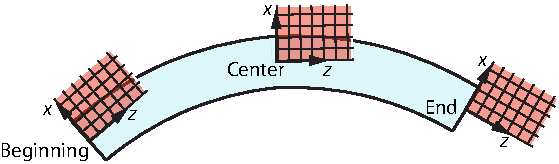
\includegraphics{bend-grid-coords.pdf}
  \caption[\vn{Field map} coordinates when used with a bend element.]{
When used with a bend element, by default, field map coordinates will be Cartesian and not
curved like the reference orbit. The orientation of the field map coordinates is
determined by the setting of \vn{ele_anchor_pt}. To use curvilinear coordinates instead,
\vn{curved_ref_frame} must be set to \vn{True} [Available in \vn{grid_field} and
\vn{taylor_field} only].}
  \label{f:bend.grid}
\end{figure}

This section explains some of the attributes that are common to the \vn{field map}
types. Not all attributes are used in all field map types. See the documentation on the
individual types for a list of the attributes pertainent to that type.

\index{field_type}
\index{field_scale}\index{master_parameter}
  \begin{description}
  \item[curved_ref_frame] \Newline
For bends, the coordinates of the field are, by default, Cartesian and do not follow the
curved bend coordinates. The orientation of the field map coordinates with respect to the
bend is determined by the placement of the anchor point (specified by \vn{ele_anchor_pt})
as shown in \fig{f:bend.grid}. In this case, when tracking a particle, \bmad will convert
particle coordinates (which are expressed in the bend's curvilinear coordinate system
defined by the reference orbit) to the Cartesian coordinates of the field map and will
rotate the computed field from the field map coordinates back to the particle coordinates.

For \vn{grid_field} and \vn{taylor_field} types only, this default behavior can be changed by
setting the \vn{curved_ref_frame} component of the field map to \vn{True}. In this case,
the field grid coordinates will follow curved bend coordinates.  The \vn{curved_ref_frame}
parameter is only pertinent for bend elements (\vn{sbend}s, \vn{rbend}s).  The setting of
\vn{curved_ref_frame} is ignored for non-bend elements.
  \item[ele_anchor_pt] \Newline
The \vn{ele_anchor_pt}, along with \vn{r0}, determines the origin of the field with
respect to the lattice element. Possible settings are:
\begin{example}
  beginning   ! Beginning of element (default).
  center      ! Center of element.
  end         ! Exit end of element.
\end{example}
Example:
\begin{example}
  rfc0: rfcavity, taylor_field = \{ele_anchor_pt = center, ...\}, ...
\end{example}
  \item[field_type] \Newline
The \vn{field_type} attribute sets the type of field described. Possible settings for
\vn{field_type} are:
\begin{example}
  electric      ! Pure electric field. For DC fields only.
  magnetic      ! Pure magnetic field. For DC fields only.
  mixed         ! Mixed EM fields. For AC fields and DC \vn{grid_field}.
\end{example}
Example:
\begin{example}
  bb: sbend, cartesian_map = \{field_type = electric, ...\}, ...
\end{example}
The \vn{cylindrical_map} type does not have a \vn{field_type} since it has explicit arrays
for the electric and magnetic fields.
  \item[field_scale] \Newline
The \vn{field_scale} attribute is used to scale the overall field magnitude. The default
value is 1. A value of -1 will reverse the field. If the \vn{master_parameter} is
defained, it is multiplied with the \vn{field_scale} to give the overall scale.
Example:
\begin{example}
  qq, quadrupole, grid_field = \{field_scale = 0.5, ...\}, ...
  qq[grid_field(1)%field_scale] = 0.7  ! Change field_scale value after element def.
\end{example}
  \item[harmonic] \Newline
The \vn{harmonic} attibute, along with \vn{rf_frequency} element attribute, sets the
oscillation frequency of the field map. The \vn{harmonic} attribute is only used with
\vn{cylindrical_map} and \vn{grid_field} types. The default value of \vn{harmonic} is 0.
The \vn{harmonic} number needs to be 0 for DC fields. Example:
\begin{example}
  lc1: lcavity, rf_frequency = 500e6, grid_field = \{harmonic = 2, ...\}, ...
\end{example}
Notice that \vn{rf_frequency} is set outside of any field map and is common to all field maps.
  \item[master_parameter] \Newline
The \vn{master_parameter} defines a ``master'' element attribute for scaling the field. Example:
\begin{example}
  qq: quadrupole, taylor_field = \{master_parameter = 'K1', ...\}, k1 = ...
\end{example}
This example defines the \vn{master_parameter} for the \vn{taylor_field} to be the
quadrupole strength \vn{k1}. By using the same master parameter for a set of field map
instances within a given lattice element, the sum field of the set can be controled by a
single attribute. The \vn{master_parameter} must be set to a valid element attribute. If
the name is blank (""), no master parameter is used. The \vn{master_parameter}, if
defined, is multiplied with the \vn{field_scale} to give the value used to scale the
fields. The default \vn{master_parameter} is blank ("") except for \vn{wiggler} elements
where, for historical reasons, the default is \vn{polarity}.

Certain parameters have an associated ``error'' parameter. If the \vn{master_parameter} is one of
these parameters, the value used to scale the field is the sum of the \vn{master_parameter} and the
associated error parameter. The elements that have associated error parameters are:
\begin{example}
  Parameter     Assoc. Error Param    Element Type
  ---------     ------------------    --------------
  Voltage       Voltage_err           E_gun, LCavity
  Gradient      Gradient_err          E_gun, LCavity
  Phi0          Phi0_err              E_gun, LCavity
  G             G_err                 Sbend, Rbend
  B_field       B_field_err           Sbemd, Rbend
\end{example}
  \item[phi0_fieldmap] \Newline
For AC fields, \vn{phi0_fieldmap} is the phase of the field map field relative to the fundamental
mode. The phase \vn{phi0_fieldmap} is relative to the fundamental frequency and not the frequency of
the field map mode. That is, the ``zero crossing'' point of the field map is shifted by a time
\vn{phi0_fieldmap}/$f_0$ where $f_0$ is the fundamental mode frequency.
  \item[r0] \Newline
The \vn{r0} attribute is the $(x0, y0, z0)$ vector specifying the offset of the origin point
that defines the field relative to the \vn{anchor} point defined by \vn{ele_anchor_pt}.
The origin position of the field (\vn{r_origin}) is determined by 
\begin{example}
  r_origin = r0 + r_anchor
\end{example}
where \vn{r_anchor} is determined by the setting of \vn{ele_anchor_pt}. In the reference
coordinates (\sref{s:ref}) with respect to the element \vn{r_anchor} is:
\begin{example}
  ele_anchor_pt       r_anchor
  -------------       ---------
  beginning           (0, 0, 0)      ! Default
  center              (0, 0, L/2)
  end                 (0, 0, L)
\end{example}
with \vn{L} being the length of the element. 

Example:
\begin{example}
  rfc0: rfcavity, taylor_field = \{r0 = (-0.23, ...), ...\}, ...
\end{example}
  \end{description}

%-----------------------------------------------------------------
\subsection{Cartesian_Map Field Map}
\label{s:cart.map}
\index{cartesian_map}

The \vn{cartesian_map} field map is only used for DC fields. Each term of a
\vn{cartesian_map} is a solution of Laplace's equation in cartesian coordinates.
as described in Sec.~\sref{s:cart.map.phys}. 

The lattice file syntax for the \vn{cartesian_map} type is:
\begin{example}
  cartesian_map = \{
    field_type       = <String>,           ! Type of field: Default = Magnetic.
    field_scale      = <Real>,             ! Scale factor for the E & B fields.
    master_parameter = <Name>,             ! Master scaling parameter for E & B fields.
    ele_anchor_pt    = <Position>,         ! Anchor position: Beginning (default), Center, or End.
    r0               = (<x0>, <y0>, <z0>), ! Anchor offset. Default is 0.
    term = \{<A>, <k_x>, <k_y>, <k_z>, <x_0>, <y_0>, <phi_z>, <family>\}, 
    term = \{....\}  \}
\end{example}
The possible settings of \vn{<family>} are explained in Sec.~\sref{s:cart.map.phys}.
Example:
\begin{example}
  q01: quadrupole, l = 0.6, field_calc = fieldmap,
        cartesian_map = \{
          term = \{0.03, 3.00, 4.00, 5.00, 0, 0, 0.63, y\},
          term = \{...\}, ...    \}
\end{example}

See Sec.~\sref{s:fieldmap.com} for an explanation of the attributes that are common with
other field map types. 

To use with PTC dependent tracking methods (\sref{s:integ}) there are a number of
restrictions: 
  \begin{itemize}
  \item
There can be only one \vn{cartesian_map} field map and there cannot be any other field
maps of any kind.
  \item 
\vn{cartesian_map} may not be used with a bend.
  \item
Only magnetic fields may be used. 
  \item
The transverse terms in \vn{r0} must be zero.
  \end{itemize}

%-----------------------------------------------------------------
\subsection{Cylindrical_Map Field Map}
\label{s:cylind.map}
\index{ccylindrical map}

The \vn{cylindrical_map} field map is used for both DC and AC fields. Each term of a
\vn{cylindrical_map} is a solution of Laplace's equation in cylindrical coordinates.
as described in Sec.~\sref{s:cylind.map.phys}. 

The lattice file syntax for the \vn{cylindrical_map} type is:
\begin{example}
  cylindrical_map = \{
    field_scale      = <Real>,             ! Scale factor for the E & B fields.
    master_parameter = <Name>,             ! Master scaling parameter for E & B fields.
    ele_anchor_pt    = <Position>,         ! Anchor position: Beginning (default), Center, or End.
    m                = <Integer>,          ! Azimuthal mode number
    harmonic         = <Integer>,          ! RF frequency harmonic number 
    phi0_fieldmap    = <Real>,             ! Phase of oscillations.
    theta0_azimuth   = <Real>,             ! Azimuthal orientation.
    r0               = (<x0>, <y0>, <z0>), ! Anchor offset. Default is 0.
    dz        = <Real>,                    ! Distance between sampled field points.
    e_coef_re = (<Real>, <Real>, ....),    ! Real part of E.
    e_coef_im = (<Real>, <Real>, ....),    ! Imaginary part of E.
    b_coef_re = (<Real>, <Real>, ....),    ! Real part of B.
    b_coef_im = (<Real>, <Real>, ....),    ! Imaginary part of B.
  \}
\end{example}
See Sec.~\sref{s:fieldmap.com} for an explanation of the attributes that are common with
other field map types.

For DC fields, the \vn{e} coefficients specify the electric fields and the \vn{b} coefficients
specify the magnetic fields. For AC fields, the \vn{e} coefficients specify modes that have finite
longitudinal electric fields while the modes associated with the \vn{b} coefficients do not.

To specify the RF frequency, specify the \vn{rf_frequency} {\em element} attribute along with
the \vn{harmonic} attribute. See the discussion of the \vn{harmonic} attribute in 
Sec.~\sref{s:fieldmap.com}.

The basic equations used for the \vn{cylindrical_map} decomposition of the fields are given in
Section~\sref{s:cylind.map.phys}. A lattice element may have multiple \vn{cylindriacl_map}
components with each \vn{cylindrical_map} being associated with a particular azimuthal mode $m$.

\vn{e_re} and \vn{e_im} give the real an imaginary part of $e$ and \vn{b_re} and \vn{b_im} give the
real and imaginary part of $b$. All of these vectors must be present and have the same length. The
exception is with an $m = 0$ mode either the $e$ or $b$ arrays can be omitted and will default to
zero. The number of terms $N$ for the $e$ or $b$ vectors must be a power of $2$ and all modes must
have the same number of terms. The $n$\Th element in the $e$ or $b$ arrays, with $n$ running from 0
to $N-1$, is associated with a wavelength $k_n$
\begin{equation}
  k_n = \begin{cases}
    \frac{2 \, \pi \, n}{N \, dz} & 0 \le n < \frac{N}{2} \\
    \frac{2 \, \pi \, (n-N)}{N \, dz} & \frac{N}{2} \le n \le N - 1
  \end{cases}
\end{equation}
This convention produces less high frequency components then the convention of using $k_n = 2 \, \pi
\, n / N dz$.

The longitudinal length of the field is
\begin{equation}
  L_{\text{field}} = \frac{N - 1}{dz}
\end{equation}
this may be different from the length \vn{l} specified for the element.

For AC fields, the time $t$ in \Eq{eseei} is computed depending upon whether \vn{absolute time
tracking} or \vn{relative time tracking} is being used as discussed in \sref{s:rf.time}. For
\vn{rfcavity} elements, the phase factor $\phi_{0j}$ in \Eq{eseei} is computed by
\begin{example}
  \(\phi_{0j}\) = harmonic(j) * [0.25 - (phi0 + phi0_multipass + phi0_err + 
                                                  phi0_autoscale + phi0_fieldmap(j))] 
\end{example}
where \vn{phi0_fieldmap(j)} and \vn{harmonic(j)} are specific to the j\Th grid field
while the other factors are element parameters and so will be the same for all grid field
maps of a given element. For non \vn{rfcavity} elements the phase is
\begin{example}
  \(\phi_{0j}\) = harmonic(j) * [phi0 + phi0_multipass + phi0_err + 
                                                  phi0_autoscale + phi0_fieldmap(j)]
\end{example}
where \vn{phi0_fieldmap(j)} and \vn{harmonic(j)} are specific to the j\Th cylindrical field map
while the other factors are element parameters and so will be the same for all cylindrical field
maps of a given element.

Example:
\begin{example}
  m1: lcavity, rf_frequency = 1e6, voltage = 2e6, cylindrical_map = \{
    m = 2,                   harmonic = 3,
    r0 = (0, 0, 0.001),      dz = 0.1,
    theta0_azimuth = 0.3,    field_scale = 0.7,
    ele_anchor_pt = center,  master_parameter = voltage,
    e_coef_re = (...),       e_coef_im = (...),
    b_coef_re = (...),       b_coef_im = (...)\}, field_calc = fieldmap
\end{example}

Note: When using PTC based tracking (\sref{c:methods}), the following restrictions apply:
\begin{Itemize}
\item
The fields must be DC.
\item
all the \vn{e_coef} and \vn{b_coef} arrays must have the same length.
\item
\vn{r0(1)} and \vn{r0(2)} (the transverse offsets) must be zero.
\item
The element containing the map cannot be an \vn{sbend} or \vn{rbend}.
\item
May not be combined with other field map types.
\end{Itemize}

%-----------------------------------------------------------------
\subsection{Grid_Field Field Map}
\label{s:grid.field}
\index{grid field}

A \vn{grid_field} is grid of field points specified using the syntax:
\begin{example}
  grid_field = \{ 
    geometry         = <String>,    ! Geometry of the grid.
    field_type       = <String>,    ! Type of field: Default = Mixed.
    field_scale      = <Real>,      ! Scale factor for the E & B fields.
    phi0_fieldmap    = <Real>,      ! Phase of oscillations.
    harmonic         = <Integer>,   ! RF frequency harmonic number 
    master_parameter = <Name>,      ! Master scaling parameter for E & B fields.
    curved_ref_frame = <Logical>,   ! Use a curved reference frame with bends?
    r0   = (...),                   ! Grid origin. Syntax is \vn{geometry} dependent.
    dr   = (...),                   ! Grid spacing. Syntax is \vn{geometry} dependent.
    ele_anchor_pt = <Position>      ! BEGINNING, CENTER, or END
    pt(<Integer>, \dots) = ( \ldots ), ! Field points. Syntax is \vn{geometry} dependent.
    \ldots \} \} \}
\end{example}
See Sec.~\sref{s:fieldmap.com} for an explanation of the attributes that are common with
other field map types.

To specify the RF frequency, specify the \vn{rf_frequency} {\em element} attribute along with
the \vn{harmonic} attribute. See the discussion of the \vn{harmonic} attribute in 
Sec.~\sref{s:fieldmap.com}.

For \vn{field_type} set to \vn{electric} or \vn{magnetic}, the field is DC. That is, For
\vn{field_type} set to \vn{electric} or \vn{magnetic}, the value of \vn{harmonic} must be
0. For \vn{field_type} set to \vn{mixed}, the field may be DC or AC. 

For AC fields, the individual field components are complex.  the syntax for specifying a complex
number is:
\begin{example}
  (<Re>, <Im>)
\end{example}
Example:
\begin{example}
  pt(0, 0, -7) = ((0.34, -4.3), (2.37, 9.34), ...)  ! Complex field
  pt(0, 0, -7) = (0.12, -0.33, ...)                 ! Imaginary components are zero
\end{example}

The actual fields $\bfE$ and $\bfB$ are computed from the complex fields $\bfE_c$ and $\bfB_c$ via
\Begineq
  \bfE = \Re \Bigl[ \bfE_c \exp \left( -2 \, \pi \, i \, (\phi_t + \phi_\text{ref}) \right) \Bigr]
\Endeq
with a similar equation for $\bfB$. $\phi_t$ is the part of the phase due to when the particle
arrives at the cavity and depends upon whether \vn{absolute time tracking} or \vn{relative time
tracking} is being used as discussed in \sref{s:rf.time}. The phase $\phi_{\text{ref}}$ for the
$j$\Th grid field in an \vn{rfcavity} element is
\begin{example}
  \(\phi_\text{ref,j}\) = harmonic(j) * [0.25 - (phi0 + phi0_multipass + phi0_err + 
                                                  phi0_autoscale + phi0_fieldmap(j))] 
\end{example}
where \vn{phi0_fieldmap(j)} and \vn{harmonic(j)} are specific to the j\Th grid field
while the other factors are element parameters and so will be the same for all grid field
maps of a given element. For non \vn{rfcavity} elements the phase is
\begin{example}
  \(\phi_\text{ref,j}\) = harmonic(j) * [phi0 + phi0_multipass + phi0_err + 
                                                  phi0_autoscale + phi0_fieldmap(j)]
\end{example}

The \vn{geometry} switch sets the type of the grid and must come before
any \vn{pt} is given. The possible settings of \vn{geometry} are:
\begin{example} 
  rotationally_symmetric_rz
  xyz
\end{example}

The \vn{rotationally_symmetric_rz} setting for \vn{geometry} is for fields
that are rotationally symmetric around the $z$ axis. The format for
this type of \vn{grid_field} is
\begin{example}
  grid_field = \{ 
    geometry = rotationally_symmetric_rz,
    r0   = (<x0>, <y0>, <z0>),  ! Grid origin 
    dr   = (<dr>, <dz>),        ! Grid spacing
    pt(<ir>, <iz>) = (<E_r>, <E_phi>, <E_z>) ! For field_type = Electric
    pt(<ir>, <iz>) = (<B_r>, <B_phi>, <B_z>) ! For field_type = Magnetic
    pt(<ir>, <iz>) = (<E_r>, <E_phi>, <E_z>, <B_r>, <B_phi>, <B_z>)
                                             ! For field_type = Mixed.
    \ldots \} 
\end{example}
where \vn{<iz>} can be negative but \vn{<ir>} must be non-negative.  

The \vn{xyz} setting for \vn{geometry} can be used for all rectangular field grids. The
format for this type of \vn{grid_field} is
\begin{example}
  grid_field = \{ 
    geometry = xyz,
    r0   = (<x0>, <y0>, <z0>),    ! Grid origin 
    dr   = (<dx>, <dy>, <dz>),    ! Grid spacing
    pt(<ix>, <iy>, <iz>) = (<E_x>, <E_y>, <E_z>),  ! For field_type = Electric
    pt(<ix>, <iy>, <iz>) = (<B_x>, <B_y>, <B_z>),  ! For field_type = Magnetic
    pt(<ix>, <iy>, <iz>) = (<E_x>, <E_y>, <E_z>, <B_x>, <B_y>, <B_z>), 
                                                   ! For field_type = Mixed.
    \ldots \}
\end{example}
where \vn{<ix>}, \vn{<iy>}, and \vn{<iz>} can be negative.

[For clarity sake, the following discusses the \vn{xyz} case. Extension to other cases is
straight forward.]  There is no restriction on the bounds of the indexes \vn{(ix, iy, iz)}
of the \vn{pt(ix, iy, iz)} array. A point $(ix, iy, iz)$ corresponds in space to the point
$(x, y, z)$:
\begin{example}
  (x, y, z) = dr * (ix, iy, iz) + r0 + r_anchor
\end{example}
where \vn{z} is measured from the beginning of the element and
\vn{r_anchor} is determined by the setting of \vn{ele_anchor_pt}:
\begin{example}
  ele_anchor_pt       r_anchor
  -------------       ---------
  beginning           (0, 0, 0)      ! Default
  center              (0, 0, L/2)
  end                 (0, 0, L)
\end{example}
with \vn{L} being the length of the element. 

Example:
\begin{example}
  apex: e_gun, l = 0.23, field_calc = fieldmap, rf_frequency = 187e6, 
                                  grid_field = call::apex_gun_grid.bmad
\end{example}
with the file \vn{apex_gun_grid.bmad} being:
\begin{example}
  \{
    geometry = rotationally_symmetric_rz,
    harmonic = 1,
    master_parameter = voltage,
    r0 = (0, 0),
    dr = (0.001, 0.001),
    pt(0,0) = ( (0, 0), (0, 0), (1, 0),  (0, 0), (0, 0), (0, 0)),
    pt(0,1) = ( (0, 0), (0, 0), (0.99, 0),  (0, 0), (0, 0), (0, 0)),
    ... \}
\end{example}

It is considered an error if the field of the grid is evaluated for a point that is transversely
outside of the grid. That is, a grid must extend transversely to the aperture or at least beyound
the trajectory of any particle. [Actually, to prevent problems when the aperture is set at the grid
boundary, if the distance between the particle and the grid boundary is within 1/2 of the spacing
between grid points, no error is generated and the field will calcuated using extrapolation.] On the
other hand, it is acceptable to evaluate the grid field at a point that is longitudinally outside of
the grid. In this case, the field is assumed to go to zero. This is done by effectively adding to
the grid two planes of zero field longitudinally to either side of the grid. So a particle traveling
ouside of the grid longitudinally will see the field drop to zero within one longitudinal grid
spacing length.

%-----------------------------------------------------------------
\subsection{Taylor_Field Field Map}
\label{s:taylor.field}
\index{taylor field}

The \vn{taylor_field} field map is only used for DC fields. A \vn{taylor_field} is comprised
of a set of two dimensional Taylor maps.  

The syntax for describing a \vn{taylor_field} is:
\begin{example}
  taylor_field = \{
    field_type       = <String>,           ! Type of field: Default = Magnetic.
    field_scale      = <Real>,             ! Scale factor for the E & B fields.
    master_parameter = <Name>,             ! Master scaling parameter for E & B fields.
    curved_ref_frame   = <Logical>,        ! Use curved coords with bends?
    canonical_tracking = <logical>         ! Use (px, py) instead of (x', y') when tracking?
    ele_anchor_pt    = <Position>,         ! Anchor position: Beginning (default), Center, or End.
    r0               = (<x0>, <y0>, <z0>), ! Anchor offset. Default is 0.
    dz               = <Real>,             ! Distance between sampled field points.
    plane(<i>) = \{<term1>, <term2>, <term3>, ....\}, ! Taylor map at constant z.
    plane(<j>) = \{....\}  \}
\end{example}
See Sec.~\sref{s:fieldmap.com} for an explanation of the attributes that are common with
other field map types.

Each \vn{plane(<i>)} component specifies a Taylor map at constant z
(\sref{s:taylor.field.phys}). The index \vn{<i>} for the different planes must be in
consecutive order. The plane with <i> = 0 corresponds to the $z = 0$ origin. There is no
restriction for the starting \vn{<i>} index of the first plane. That is, there does not
have to be a plane with index \vn{<i>} = 0 (in this case, the origin needs to be outside
of the element).

The individual Taylor series terms follow the same syntax as the Taylor terms in a
\vn{taylor} element (\sref{s:taylor}):
\begin{example}
  \{<out>: <coef>, <e1> <e2>\}           ! EM Taylor term. First form.
  \{<out>: <coef> | <n1> <n2> ...\}      ! EM Taylor term. Second form.
\end{example}
except that 1) \vn{<out>} must be one of
\begin{example}
  Bx, By, or Bz
\end{example}
2) there are only two exponents \vn{<e1>} and \vn{<e2>}
corresponding to \vn{x}, and \vn{y} respectively for the first form,  and 3) the integers
\vn{<n1>}, \vn{<n2>}, etc., are restricted to being 1 or 2.

To use with PTC dependent tracking methods (\sref{s:integ}) there are a number of
restrictions: 
  \begin{itemize}
  \item
There can be only one \vn{taylor_field} field map and there cannot be any other field
maps of any kind.
  \item 
The number of planes must be odd. If you want to be able to track with PTC to the center
of the element, the number of planes must be of the form $4 \, n + 1$ where $n$ is an
integer.
  \item
Only magnetic fields may be used.
  \item
The plane locations must be symmetric with respect to the center of the element. That is,
the first plane and the last plane must be equidistant from the element center.
  \item
The element may not be superimposed upon (\sref{s:super}). [PTC tracks from plane to plane
so there is no good way to cut an element at an arbitrary position.]
  \item
In a bend with \vn{curved_ref_frame} = False, The setting of \vn{ele_anchor_pt} must be
\vn{center}.
  \end{itemize}
If the edges of the \vn{taylor_field}, which are defined by the first and last planes, is
different than the edges of the element, \bmad and PTC will do tracking differently. With
\bmad, the tracking will start at one edge of the element and will end at the other
end. That is, \bmad will ignore the field outside of the element (but this can be modified
using field overlap (\sref{s:overlap})). PTC, on the other hand, will start at an element
end and then track from the element end backwards to the first plane like in a drift. It
will then track to the ending plane and finally track backwards from the ending plane to
the ending element edge line in a drift. That is, PTC does not ignore the field outside of
the element.

When using PTC based tracking (\sref{c:methods}), the \vn{canonical_tracking} parameter
can be used to select whether the transverse phase space coordinates used in tracking is
the canonical $(x, p_x, y, p_y)$ (\sref{s:phase.space}) coordinates or the non-canonical
$(x, x', y, y')$ coordinates. The default is \vn{False}. The difference comes at the edges
of element if the field is not zero. With canonical coordinates, there is a kick at the
edge while with the non-canonical there is not. What is best depends upon the problem. For
example, with a solenoid magnet where the field is constant right up to the edge,
canonical tracking will be needed since the edge kick is significant. However, the edge
kick is not well defined (that is, certain assumptions are built into the edge kick
calculation. For example, with a solenoid, cylindrical symmetry is generally
assumed). Thus for some arbitrary field, the assumptions used by PTC may by incorrect for
the problem at hand. Thus in many cases, especially for single pass machines, the
non-canonical tracking is a better choice.

Example:
\begin{example}
  t1: sbend, k1 = 2, taylor_field = \{
    field_type = electric,   ele_anchor_pt = end, 
    dz = 1.2,                r0 = (0, 0, 2.0),
    field_scale = 1.3,       curved_ref_frame = False,
    master_parameter = k1,
    plane(-2) = \{\{Bx: 0.3| 1\}, \{Bx: 1.3, 1 2\}, \{By: 0.7, 3 1\}, ...\},
    plane(-1) = \{\{Bx: 0.6|\}, \{By: 0.4|112\}, \{By: 0.7, 4 0\}, ...\}, 
    ...  \}, field_calc = fieldmap
\end{example}

%-----------------------------------------------------------------
\section{RF Couplers}
\label{s:rf.coupler}

\index{lcavity}\index{rfcavity}
\index{coupler_at}\index{coupler_strength}
\index{coupler_angle}\index{coupler_phase}
For \vn{lcavity} and \vn{rfcavity} elements, the attributes that
characterize the dipole transverse kick due to a coupler port are:
\begin{example}
  coupler_at       = <Switch> ! What end the coupler is at
  coupler_strength = <Real>   ! Normalized strength
  coupler_angle    = <Real>   ! Polarization angle (rad/2\(\pi\))
  coupler_phase    = <Real>   ! Phase angle with respect to the RF (rad/2\(\pi\))
\end{example}
The possible \vn{coupler_at} settings are:
\begin{example}
  entrance_end
  exit_end  ! default
  both_ends
\end{example}
The kick due to the coupler is
\begin{example}
  dP_x = amp * cos(phase) * cos(angle) 
  dP_y = amp * cos(phase) * sin(angle)
  dE   = amp * (cos(angle) * x + sin(angle) * y) * sin(phase) * twopi * rf_frequency / c_light 
\end{example}
where \vn{dP_x} and \vn{dP_y} are the transverse momentum kicks, \vn{dE} is an energy kick, and
\begin{example}
  amp   = gradient * coupler_strength 
  phase = twopi * (phase_particle + phase_ref + coupler_phase)         ! For lcavity \sref{s:lcav}
        = pi/2 + twopi * (phase_particle - phase_ref + coupler_phase)  ! For rfcavity \sref{s:lcav}
  angle = twopi * coupler_angle
\end{example}
The energy kick is needed to keep things symplectic. 

Example:
\begin{example}
  rf1: lcav, l = 4.5, gradient = 1.2e6, coupler_at = both_ends,
                                                  coupler_strength = 0.037
\end{example}

%-----------------------------------------------------------------
\section{Field Extending Beyond Element Boundary}
\label{s:overlap}

\index{field_overlaps} 
The \vn{field_overlaps} element attribute can be used to indicate that the electric or
magnetic fields of one element overlap another element. The syntax is:
\begin{example}
  <overlapping_ele>: ... field_overlaps = \{<overlapped_ele1>, <overlapped_ele2>, ...\}
\end{example}
The \{\} braces are optional if there is only one overlapped element.

Example:
\begin{example}
  b1: sbend, l = 2.3, field_overlaps = \{q1, s2\}, ...
  inj_line: line = (..., s2, b1, mark3, q1, ...)
\end{example}
In this example, the field of element \vn{b1} extends beyond the ends of \vn{b1} and
overlaps elements \vn{q1} and \vn{s2}. There is no limit to the number of elements that
are overlapped by any given element and overlapped elements do not have to be next to the
overlapping element in the line. If there are multiple elements whose name matches the
name of a overlapped element, the element closest to the overlapping element is
chosen. Thus in the above example, if there are multiple elements named \vn{q1}, the
closest \vn{q1} to \vn{b1} is designated as the overlapped element.

There can be multipole \vn{field_overlaps = ...} constructs for an overlapping element.
Thus the following is equivalent to the above example:
\begin{example}
  b1: sbend, l = 2.3, field_overlaps = q1, field_overlaps = s2
\end{example}

Note: When the field overlaps elements that are superimposed (\sref{s:super}), the overlapped 
elements must be the \vn{super_lord} elements and never the slaved elements.

The field, when \vn{field_calc} (\sref{s:integ}) is set to \vn{bmad_standard}, never extends beyond the
element boundary and so a \vn{bmad_standard} field will never overlap another element.

%-----------------------------------------------------------------
\section{Automatic Scaling of Accelerating Fields}
\label{s:autoscale}
\index{automatic field scaling|hyperbf}

\index{e_gun}\index{em_field}\index{lcavity}\index{rfcavity}
Elements that have accelerating fields are:
\begin{example}
  e_gun       ! \sref{s:e.gun}
  em_field    ! \sref{s:em.field}
  lcavity     ! \sref{s:lcav}
  rfcavity    ! \sref{s:rfcav}
\end{example}
[Notice that \vn{rfcavity} elements by definition, have a constant reference energy while
with all the other elements the entrance end reference energy will, in general, be
different from the exit end reference energy.]

The problem that arises with accelerating fields is how to set the overall amplitude (and
phase if the fields are oscillating) of the field so that a particle, starting on the
reference orbit and starting with the reference energy, has the desired energy gain at the
exit end of the element where the ``desired'' is set by the \vn{voltage} or \vn{gradient}
attribute of the element plus a \vn{phi0} phase attribute for AC fields.

The scaling problem is not present when \vn{bmad_standard} tracking (\sref{s:tkm}) is used
since \vn{bmad_standard} tracking uses an integrated formula that is designed to give the
proper acceleration. Rather it is a problem for Runge-Kutta and other methods integration
methods.

The problem becomes even more complicated at non-ultra relativistic energies where the
particle velocity is not a constant. In this case, the proper amplitude and/or phase
settings will depend upon what the incoming energy of the reference particle is.

To help with the scaling problem, \bmad has the capability to automatically
scale an accelerating field's amplitude and/or phase. The two
lattice element parameters that turn on/off auto scaling are (\sref{s:param}):
\begin{example}
  autoscale_phase      = <Logical>  ! Automatic phase scaling.
  autoscale_amplitude  = <Logical>  ! Automatic amplitude scaling.
\end{example}
The default value is True for both parameters. Example:
\begin{example}
  rf2: rfcavity, autoscale_phase = F
\end{example}

Scaling takes place during program execution when a lattice is initially created (that is,
when the lattice file is parsed) and when parameters in the lattice that would change the
scaling are varied.  The element parameters varied when autoscaling is done are:
\begin{example}
  field_autoscale       ! Amplitude scale
  phi0_autoscale        ! phase scale
\end{example}
For an \vn{rfcavity} element, the \vn{field_autoscale} parameter is set so that when the phase is
adjusted for maximum acceleration, the voltage gain of a particle on the zero orbit is equal to the
value of the element's \vn{voltage} parameter and then phi0_autoscale is shifted by approximately 90
degrees so that with \vn{phi0} equal to zero a particle on the zero orbit will not see any energy
gain through the cavity.

If no autoscaling is done, the default setting of \vn{field_autoscale} is 1 and the
default setting of \vn{phi0_autoscale} is 0.

For an \vn{rfcavity}, the autoscaling is normally done around a phase of \vn{phi0} = 0 which is
appropriate for a ring above transition since \vn{phi0} = 0 is the stable fixed point. Below
transition, the stable fixed point is at \vn{phi0} = 0.5. In this case, the \vn{bmad_com} global
parameter \vn{rf_phase_below_transition_ref} (\sref{s:bmad.common}) should be set to True so that
autoscaling is done around \vn{phi0} = 0.5. For an ultrarelativistic reference particle with speed
very nearly $c$ there is no difference in the autoscaling between \vn{phi0} = 0 and \vn{phi0} = 0.5.
However, when there are velocity variations of the particle within the cavity there will be differences
between autoscaling at the two phases.

Notice that if autoscaling is on, the \vn{field_autoscale} is adjusted so that a particle on the
zero orbit will see a field appropriate for the setting of the element's \vn{voltage} setting.
If autoscaling is off, the field is independent of the element's \vn{voltage} setting.

\vn{field_autoscale} and \vn{phi0_autoscale} are not needed and therefore ignored when
\vn{bmad_standard} tracking is done.

%-----------------------------------------------------------------
\section{Wakefields}
\label{s:wakes}

Wake fields can be specified for many elements.  The attributes that characterize the
wakes are:
\index{sr_wake_file}\index{lr_wake_file}\index{lr_freq_spread}
\begin{example}
  sr_wake_file     = <String>   ! Short range wake field definition file. (\sref{s:sr.wake.file})
  lr_wake_file     = <String>   ! Long range wake field definition file. (\sref{s:lr.wake.file})
  lr_freq_spread   = <Real>     ! RMS fractional frequency spread of the LR wake fields.
  lr_self_wake_on  = <Logical>  ! Apply longitudinal long range self-wake? Default = True.
\end{example}

The \vn{lr_freq_spread} attribute is used to randomly spread out the long range mode
frequencies among different cavities. The spread is Gaussian in shape with an RMS of
\vn{lr_freq_spread} * $F$ where $F$ is the frequency of a mode.

The \vn{lr_self_wake_on} attribute can be used to turn off the longitudinal long-range
self-wake which is the longitudinal kick on the particles of a bunch due to the wake
generated by these same particles. [The transverse self wake is always zero.] The default
setting of \vn{lr_self_wake_on} is \vn{True}. Turning off the self-wake, for example,
can be done to avoid double counting if both long-range and short-range wakes are defined.

Example:
\begin{example}
  abc: lcavity, lr_wake_file = 'lr.wake', lr_freq_spread = 0.0023, lr_self_wake_on = F
\end{example}

The formulas used to compute the wake field are given in \sref{s:wake.fields}. \bmad has
two modes for tracking particles. One mode tracks individual particles one at a time. The
other mode tracks bunches of particles. Which mode is used for a given program is decided
by the program. The wake field is ignored when tracking individual particles and only used
when tracking bunches.

%-----------------------------------------------------------------
\subsection{Short-Range Wakes}
\label{s:sr.wake.file}

\index{wakes!short-range}
The input file name for the short--range wake fields is specified
using the \vn{sr_wake_file} attribute. The file gives both monopole
longitudinal and dipole transverse wakes. An example input file is:
\begin{example}
  ! Pseudo Wake modes:
  !                      Amp       Damp          K      Phase  Polar-    Transverse_
  ! Longitudinal:      [V/C/m]     [1/m]      [1/m]     [rad]  ization   Dependence
  ! Transverse:      [V/C/m^2]     [1/m]      [1/m]     [rad]  

  &short_range_modes
    longitudinal(1) = 3.23e14     1.23e3     3.62e3     0.123
    longitudinal(2) = 6.95e13     5.02e2     1.90e3    -1.503
    .. etc ..
    transverse(1) =   4.23e14     2.23e3     5.62e3     0.789    X  linear_trailing
    transverse(2) =   8.40e13     5.94e2     1.92e3     1.455
     .. etc ..
    z_max = 1.3e-3
  /
\end{example}
Wakes are specified via a set of ``pseudo'' modes
(\sref{s:wake.short}). The magnitude of \vn{z_max} should be set to
the maximum $z$ value at which the pseudo mode fit is valid. \bmad
will check the distance between particles does not exceed \vn{z_max}.
If it does, \bmad will report an error.

\index{none}\index{x_axis}\index{y_axis}
The \vn{polarization} parameter is used to specify the wake
polarization. Possible settings for this parameter are:
\begin{example}
  none    ! Default
  x_axis  
  y_axis 
\end{example}
The \vn{polarization} name may be abbreviated.  For example, if the
\vn{polarization} is set to \vn{x_axis}, there is no vertical kick
from the pseudo mode.

\index{none}\index{linear_leading}\index{linear_trailing}
The \vn{transverse_dependence} parameter sets whether the wake kick
is linear in the offset of the leading or trailing particle or is
independent of the transverse offset.
Possible settings of this parameter are:
\begin{example}
  none              ! Default for longitudinal modes
  linear_leading    ! Default for transverse modes
  linear_trailing
\end{example}
The \vn{transverse_dependence} parameter may be abbreviated. Note: Due
to the way the wake file is parsed, if \vn{transverse_dependence} is
specified for a particular mode, \vn{polarization} must also be
specified.

For \vn{longitudinal} modes: If the \vn{transverse_dependence} is
\vn{none} (the default), then the \vn{polarization} must also be
\vn{none} (other combinations do not make sense). If the
\vn{transverse_dependence} is \emph{not} \vn{none} for a
\vn{longitudinal} mode, then the \vn{polarization} must be set
to \vn{x_axis} or \vn{y_axis}. 

Note: In a beam chamber with circular symmetry, the linear terms in
the \vn{longitudinal} wake are zero and the transverse wake has
no terms independent of the transverse offsets nor terms that
depend upon the trailing particle offset.

%-----------------------------------------------------------------
\subsection{Long-Range Wakes}
\label{s:lr.wake.file}

Equations for long-range wakes is given in \Sref{s:wake.long}.

The input file name for the long--range wake fields is specified using
the \vn{lr_wake_file} attribute. The file gives the wake modes by
specifying the frequency (in Hz), R/Q (in $\Omega$/meter$^{2m}$), Q,
and m (order number), and optionally the polarization angle (in
radians/2pi) for each cavity mode. The input uses Fortran90 namelist
syntax: The data begins with the string \vn{\&long_range_modes} and
ends with a slash \vn{/}. Everything outside this is ignored. Each
mode is labeled \vn{lr(i)} where \vn{i} is the mode index. An example
input file is:
\begin{example}
              Freq      R/Q      Q    m   Polar   b_sin  b_cos a_sin  a_cos  t_ref 
                      [Ohm/               Angle 
              [Hz]     m^(2m)]           [Rad/2pi]
  &long_range_modes
    lr(1) = 1.650e9    0.76    7.0e4  1    "unpol"
    lr(2) = 1.699e9   11.21    5.0e4  1    "0.15"
    lr(3) =    0       0.57    1.1e6  0    "unpol"
  /
\end{example}
[Note: The quotation marks are needed with some compilers and not with others.]  A
frequency of zero is used to designate wakes that are part of the fundamental accelerating
mode. \bmad needs to know if a wake is part of the fundamental mode due to timing issues
as discussed in \sref{s:rf.time}.

If the polarization angle is set to ``\vn{unpolarized}'' the mode is
taken to be unpolarized. [Note: Technically the unpolarized mode is
actually two polarized normal modes. The axes of these two normal
modes can be chosen arbitrary as long as they are at right angles to
each other.]

Two element attributes that affect the long-range wake are \vn{lr_freq_spread} and
\vn{lr_self_wake_on} as explained in \sref{s:wakes}.

After the long--range modes have been defined they can be
referenced or redefined using the notation
\begin{example}
  lr(n)%freq      ! Frequency
  lr(n)%r_over_q  ! R/Q
  lr(n)%q         ! Q
  lr(n)%angle     ! Polarization Angle
\end{example}
Example:
\begin{example}
  lcav[lr(2)%freq] = 1.1 * lcav[lr(2)%freq] ! Raise frequency by 10\%
\end{example}

Example:
\begin{example}
  rf1: lcav, l = 4.5, gradient = 1.2e6, sr_wake_file = "sr1.dat"
\end{example}

%-----------------------------------------------------------------
\section{Fringe Fields}
\label{s:fringe}
\index{fringe fields}

Lattice elements can have fringe fields at the element edges. Whether \bmad tries to model
the fringe fields using the models described below first depends upon what kind of
tracking is done. Fringe effects are {\em not} applied when an element's
\vn{tracking_method} is set to:
\begin{example}
  custom
  linear
  mad
\end{example}
Additionally, no fringe effects will be used if the \vn{tracking_method} is 
\vn{runge_kutta} or \vn{time_runge_kutta}, and the element's \vn{field_calc} (\sref{s:integ}) is
not \vn{bmad_standard}. This is done since it is assumed, in this case, that the body of the field
includes any fringe fields.

%-----------------------------------------------------------------
\subsection{Turning On/Off Fringe Effects}
\label{s:fringe.at}

\index{fringe_at}
Whether fringe fields are ignored or not is determined by the setting of the
\vn{fringe_at} element parameter. The possible settings are
\begin{example}
  no_end         
  both_ends             ! Default
  entrance_end
  exit_end
\end{example}
This is particularly useful in vetoing the fringe effect in the interior of split
elements. If there is no fringe at a particular boundary, the setting of attributes
like \vn{fringe_type} (see below) are ignored.

\index{spin_fringe_on}
When a particle's spin is being tracked through the fringe field at an element's edge,
the \vn{spin_fringe_on} logical attribute of the element determines how the tracking is handled.
Example:
\begin{example}
  q: quad, spin_fringe_on = T, fringe_at = exit_end
\end{example}
Here, there is no fringe effect at the entrance of the element and the fringe at the exit
end of the element will affect the spin. The default setting of \vn{spin_fringe_on} is
\vn{True}.

%-----------------------------------------------------------------
\subsection{Fringe Types}
\label{s:fringe.trype}

\bmad and PTC have several fringe field models for the magnetic field. Which fringe
model is used is set by two element attributes:
\begin{example}
  fringe_type
  ptc_fringe_geometry
\end{example}

\index{fringe_type}
For elements that have a multipole type fringe field (dipole, quadrupole, etc., as opposed
to solenoid or RF fringes), the \vn{fringe_type} switch is used to select how a fringe
field is simulated.  For everything except for \vn{rbend} and \vn{sbend} elements,
\vn{fringe_type} may be set to one of:
\begin{example}
  none              ! Default 
  soft_edge_only
  hard_edge_only
  full
\end{example}
The \vn{none} setting ignores any fringe fields.  The fringe field kick is divided into
two pieces.  The first piece is called the \vn{hard edge} fringe kick and is the kick in
the limit that the longitudinal extent of the fringe is zero. The second piece is the
\vn{soft edge} fringe kick which is the fringe kick with the fringe having a finite
longitudinal extent minus the hard edge fringe kick. That is
\begin{example}
  fringe kick = hard fringe kick + soft fringe kick
\end{example}
The advantage of separating the fringe kick in this way is that the hard fringe can be
used without having to know anything about the longitudinal extent of the fringe.  In many
cases, this is a good enough approximation. Note that using the soft fringe without the
hard fringe is not physical but can be useful in understanding how the soft edge component
affects tracking. See~\sref{s:fringe.std} for details.

For \vn{rbend} and \vn{sbend} elements, the possible \vn{fringe_type}
settings are:
\begin{example}
  none
  soft_edge_only      !          SAD equivalent: fringe = 1, disfrin = 1
  hard_edge_only      !          SAD equivalent: fringe = 0, disfrin = 0
  full
  linear_edge
  basic_bend          ! Default. SAD equivalent: fringe = 0, disfrin = 1
  sad_full            !          SAD equivalent: fringe = 1, disfrin = 0
\end{example}
The \vn{basic_bend} setting, which is the default, is essentially the basic vertical focusing effect
that is present when there is a finite \vn{e1} or \vn{e2} face angle. With \vn{bmad_standard}
tracking, \vn{basic_bend} also includes second order terms (\sref{s:fringe.bend.hard}). The
\vn{linear_edge} setting ignores these second order terms.  In some cases, for instance in a
chicane, \vn{basic_bend} is not good enough. With \vn{fringe_type} set to \vn{full}, higher order
effects are taken into account.

PTC does not have a \vn{linear_edge} fringe model.
With PTC tracking, \vn{basic_bend} tracking is used if \vn{linear_edge} is chosen.

Additionally, for use with PTC, the \vn{ptc_fringe_geometry} switch can be used
to define the symmetry of the fringe fields. Possible settings are:
\begin{example}
  x_invariant
  multipole_symmetry
\end{example}
\index{ptc_max_fringe_order}
The difference between \vn{x_invariant} and \vn{multipole_symmetry} is
that with \vn{multipole_symmetry} the fringe field for an $n$\Th order
multipole is assumed to have the same rotational symmetry as the
multipole. With this assumption, the fringe field has $n+1$\St order
terms.  With \vn{x_invariant}, the fringe field is calculated assuming
that there is translational invariance along the horizontal $x$
axis. This differs from \vn{multipole_symmetry} by adding terms of
increasing order consistent with the translational invariance. See
\'Etienne Forest's book\cite{b:forest} for more details. Which setting
of \vn{ptc_fringe_geometry} is appropriate depends upon how the dipole
under consideration is constructed. The two settings of
\vn{ptc_fringe_geometry} represent two points of a continuum of
possible fringe field geometries.

Additionally, when using PTC tracking (\sref{s:ptc.intro}), the
\vn{parameter[ptc_max_fringe_order]} (\sref{s:param}) determines the
maximum order of the calculated fringe fields.

Example:
\begin{example}
  b1: rbend, angle = pi/4, g = 0.3, fringe_type = full
\end{example}

In a bend element, the \vn{fringe_type} setting only pertains to the
dipole fringe.  For higher order multipole fields in a bend, the
\vn{higher_order_fringe_type} selects the fringe type. Possible
settings are the same as for the non-bend \vn{fringe_type} elements
\begin{example}
  none              ! Default 
  soft_edge_only
  hard_edge_only
  full
\end{example}

\index{sad}\index{sbend}\index{rbend}
The \vn{soft_edge_only}, \vn{hard_edge_only} and \vn{sad_full} settings
of \vn{fringe_type} emulate the fringe field tracking used in the SAD
program\cite{b:sad}.  The \vn{soft_edge_only} setting only uses the linear
part of the fringe, \vn{hard_edge_only} ignores the linear part of
the fringe, and \vn{sad_full} uses the full fringe.  For an \vn{sbend}
or \vn{rbend} element, these SAD fringe fields are in addition to the
fringe fields that occurs with a finite \vn{e1} or \vn{e2} face
angle. 

For \vn{quadrupole} and \vn{sad_mult} elements, the translation between the \vn{fringe_at}
and \vn{fringe_type} settings and the \vn{fringe} and \vn{disfrin} switches of SAD is:
\begin{center}
\tt
\begin{tabular}{ll|llll} 
              &                      & \multicolumn{4}{c}{fringe_at:} \\
              &                      & no_end     & entrance_end & exit_end   & both_ends$^*$ \\ \midrule
\multirow{4}{*}{fringe_type:} 
              & none                 & [0, $\ne 0$] & [0, $\ne 0$]   & [0, $\ne 0$] & [0, $\ne 0$] \\
              & soft_edge_only       & [0, $\ne 0$] & [1, $\ne 0$]   & [2, $\ne 0$] & [3, $\ne 0$] \\
              & hard_edge_only$^*$   & [0, $\ne 0$] & No SAD Equiv   & No SAD Equiv & [0, $= 0$]   \\
              & full                 & [0, $\ne 0$] & [1, $= 0$]     & [2, $= 0$]   & [3, $= 0$]   \\ 
  \bottomrule
\multicolumn{2}{l}{$^*$Default value.} & \multicolumn{4}{l}{\textbf{[fringe, disfrin]}} \\
\end{tabular}
\end{center}
Each entry is the table is of the form [\vn{fringe}, \vn{disfrin}]. The
\vn{soft_edge_only} fringe kick is a kick that is linear in the transverse $(x, p_x, y,
p_y)$ coordinates and comes from the finite width of the quadrupolar fringe field. The
width of the quadrupolar fringe field is characterized by the \vn{f1} and \vn{f2}
attributes. The \vn{sad_nonlinear_only} fringe kick comes from the nonlinear part of the
quadrupolar field plus the fringes of the other multipoles.

The soft fringe quadrupole parameters \vn{fq1} and \vn{fq2} (\sref{s:q.soft}) are related
to the corresponding SAD parameters \vn{f1} and \vn{f2} via
\begin{example}
  f1 = -sign(fq1) * sqrt(24 * |fq1|)
  f2 = fq2
\end{example}
In the SAD documentation, the soft edge is called the ``linear'' fringe.

\index{permfringe}\index{bendfringe}
For programmers who deal with PTC directly: The translation between
\vn{ptc_fringe_geometry} on the \bmad side and \vn{bendfringe} on the
PTC side is:

\begin{center}
\begin{tabular}{lll} \toprule 
{\em ptc_fringe_geometry} & {\em bendfringe} \\ \midrule
  x_invariant             & True  \\
  multipole_symmetry      & False \\ \bottomrule
\end{tabular}
\end{center}

%-----------------------------------------------------------------
\section{Instrumental Measurement Attributes}
\label{s:meas.attrib}

\index{instrument}\index{monitor}\index{marker}\index{detector}
\index{x_gain_err}\index{y_gain_err}\index{crunch}\index{noise}
\index{x_gain_calib}\index{y_gain_calib}\index{crunch_calib}
\index{x_offset}\index{y_offset}\index{tilt}
\index{x_offset_calib}\index{y_offset_calib}\index{tilt_calib}
\index{de_eta_meas}\index{n_sample}\index{osc_amplitude}

\vn{instrument}, \vn{monitor}, \vn{detector}, and \vn{marker} elements
have special attributes to describe errors associated with orbit, betatron phase, dispersion
and coupling measurements. These attributes are: \hfill\break
\hspace*{0.1in}
\begin{tabular}{lll} \toprule
  {\em Attribute}     & {\em Symbol} (See: \sref{s:meas.calc}) & \\ \midrule
  \vn{tilt}           & $\theta_t$             & See \sref{s:offset} \\ 
  \vn{x_offset}       & $x_{\text{err}}$       & See \sref{s:offset} \\ 
  \vn{y_offset}       & $y_{\text{err}}$       & See \sref{s:offset} \\ 
  \vn{x_gain_err}     & $dg_{x,\text{err}}$    & Horizontal gain error \\ 
  \vn{y_gain_err}     & $dg_{y,\text{err}}$    & Vertical gain error \\ 
  \vn{crunch}         & $\psi_{\text{err}}$    & Crunch angle \\ 
  \vn{tilt_calib}     & $\theta_{\text{err}}$  & tilt angle calibration \\ 
  \vn{x_offset_calib} & $x_{\text{cal}}$       & Horizontal offset calibration \\ 
  \vn{y_offset_calib} & $y_{\text{cal}}$       & Vertical offset calibration \\ 
  \vn{x_gain_calib}   & $dg_{x,\text{cal}}$    & Horizontal gain calibration \\ 
  \vn{y_gain_calib}   & $dg_{y,\text{cal}}$    & Vertical gain calibration \\ 
  \vn{crunch_calib}   & $\psi_{\text{cal}}$    & Crunch angle calibration \\ 
  \vn{noise}          & $n_f$                  & Noise factor \\ 
  \vn{de_eta_meas}    & $dE/E$                 & Percent change in energy \\ 
  \vn{n_sample}       & $N_s$                  & Number of sampling points \\ 
  \vn{osc_amplitude}  & $A_{\text{osc}}$       & Oscillation amplitude \\ \bottomrule
\end{tabular}
\hfill\break
A program can use these quantities to calculate ``measured'' values from the
``laboratory'' values. Here, ``laboratory'' means as calculated from some model lattice.
See \sref{s:meas.calc} for the conversion formulas.
